\section{Model Parameterization}\label{mod.par}
Model parameterization involves specification of parameter values (model inputs),
such as proportions, probabilities, rates, and ratios.
This section describes the data, analyses, and assumptions used to derive these inputs.
A summary of calibrated parameters, calibration targets, and methodology is given in \sref{mod.cal}.
%===================================================================================================
\subsection{Preliminaries}\label{mod.par.math}
%---------------------------------------------------------------------------------------------------
\paragraph{Deriving Prior Distributions}
Uncertainty distributions for most parameters and calibration targets were estimated by
fitting a parametric distribution to specified quantiles.
Let $f\,(x\mid\theta)$ be
the probability density function of random variable~$x$ (parameter or calibration target)
given distribution parameters $\theta$.
Then $F\,(x\mid\theta) = \int_0^x f(\tau)\,d\tau$ is the cumulative distribution function,
and $Q(p\mid\theta) = F^{\,-1}(p\mid\theta)$ is the quantile function.
Our objective is to estimate $\theta$, given a set of quantiles
(\eg $q = \{q_{2.5},q_{97.5}\}$ for the 95\%~CI).
For each estimation, we minimized the following error function,
using the L-BFGS-B algorithm \cite{Byrd1995}:
\begin{equation}
  J(\theta) = \sum_i {\big|\,q_i - Q(p_i\mid\theta)\,\big|}^{\,\omega}
\end{equation}
where $\omega$ can specify absolute differences ($\omega=1$) or squared differences ($\omega=2$)
to improve convergence.
Distribution fit was validated visually using a plot of
the distribution quantiles $Q(p_i\mid\theta)$ \vs the target quantiles $q_i$,
overlaid on the density distribution $f\,(x\mid\theta)$; \eg Figure~\ref{fig:distr.fit}.
\begin{figure}[h]
  \centering
  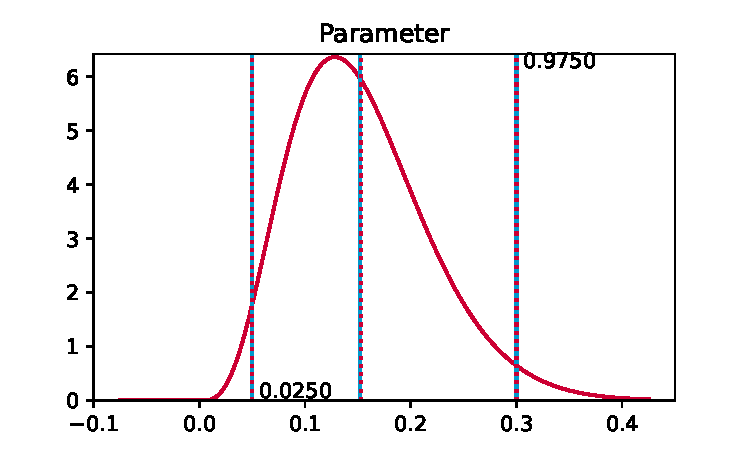
\includegraphics[width=.6\linewidth]{distr.fit}
  \caption{Example distribution fitting validation plot}
  \label{fig:distr.fit}
  \floatfoot{BAB distribution fit to $\{q_{2.5} = .05, q_{97.5} = .30\}$;
    blue solid lines: target quantiles $q_i$;
    red dotted lines: distribution quantiles $Q(p_i\mid\theta)$;
    red solid line: density distribution $f\,(x\mid\theta)$.}
\end{figure}
%---------------------------------------------------------------------------------------------------
\paragraph{Beta Approximation of the Binomial (BAB) Distribution}
Numerous model parameters and calibration targets represent population proportions.
Such proportions can be estimated as $\rho = n / N$, where
$N$ is the sample size and $n$ is the number of individuals with the characteristic of interest.
The uncertainty around $n$ is then given by the binomial distribution:
\begin{equation}\label{eq:binom}
  p(n) = {N \choose n} \, \rho^{n}{(1 - \rho)}^{N - n}
\end{equation}
However, \eqref{eq:binom} is only defined for discrete values of $n$.
It is more convenient to have a continuous distribution for $\rho$,
for sampling parameters and evaluating the likelihood of calibration targets,
since compartmental models can have non-whole-number population sizes.
For this purpose, we use a beta approximation of the binomial distribution (BAB):
\begin{equation}\label{eq:beta}
  p(\rho) =
    \frac{\Gamma(\alpha+\beta)}{\Gamma(\alpha)\,\Gamma(\beta)}\,
    \rho^{\alpha-1}{(1 - \rho)}^{\beta-1}
\end{equation}
with $\alpha = N\,\rho$ and $\beta = N\,(1-\rho)$.
Unlike the approximation by a normal distribution,
the beta distribution ensures that $\rho \in [0,1]$.
Figure~\ref{fig:bab} illustrates the approximation for
$N = \{10,20,40\}$ and $\rho = \{0.01,0.1,0.5\}$.
\begin{figure}
  \centering
  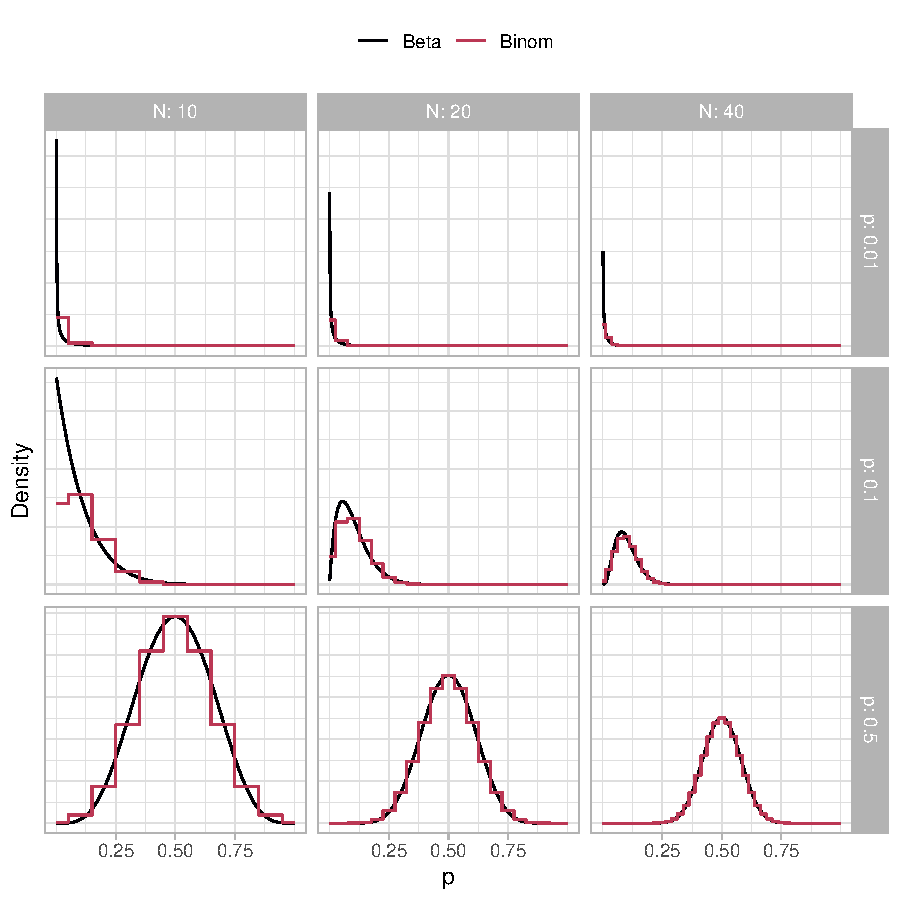
\includegraphics[width=.8\linewidth]{bab}
  \caption{Beta approximation of the binomial distribution (BAB)}
  \label{fig:bab}
\end{figure}

%===================================================================================================
\subsection{Data Sources for Eswatini}\label{mod.par.data}
Major HIV data sources for Eswatini are summarized in Table~\ref{tab:data.esw},
and briefly described as follows.
Summary statistics were extracted from reports and publications in all cases,
except two FSW surveys \cite{Baral2014,EswKP2014},
for which individual-level data were obtained and analyzed directly in \sref{mod.par.fsw}.
\begin{table}
  \centering
  \caption{Main data sources for Eswatini}
  \label{tab:data.esw}
  \begin{tabular}{llllrl}
  \toprule
  Ref & ID & Dates\tn{a} & Population\tn{b} & N\tn{c} & HIV\tn{d} \\
  \midrule
  \cite{SDHS2006}    & DHS'06 & 07/06\,--\,02/07 & GP 15+    &  9,143 & P    \\
  \cite{SHIMS1}      & SHIMS1 & 12/10\,--\,06/11 & GP 18--49 & 18,169 & P, I \\
  \cite{SHIMS2}      & SHIMS2 & 08/16\,--\,03/17 & GP 15+    &  9,146 & P, I \\
  \cite{SHIMS3}\tn{e}& SHIMS3 & 05/21\,--\,11/21 & GP 15+    & 12,043 & P, I \\
  \cite{Baral2014}   & KP'11  & 09/11\,--\,10/11 & KP 15+    &    328 & P    \\
  \cite{EswKP2014}   & KP'14  & 09/14\,--\,01/15 & KP 18+    &    781 & ---  \\
  \cite{EswIBBS2022} & KP'21  & 10/20\,--\,01/21 & KP 18+    &    676 & P, I \\
  \bottomrule
\end{tabular}
\floatfoot{
  \tnt[a]{Baseline data collection (\textsc{mm/yy})};
  \tnt[b]{GP: general population; KP: key populations (female sex workers, men who have sex with men)};
  \tnt[c]{Respondents aged xx--49 who completed baseline survey};
  \tnt[d]{Estimates of HIV via blood test, P:~prevalence, I:~incidence};
  \tnt[e]{Preliminary findings only}.}


\end{table}
%---------------------------------------------------------------------------------------------------
\paragraph{General Population}
The 2006--07 Demographic and Health Survey (DHS) \cite{SDHS2006} was
the first nationally representative, household-based survey in Eswatini
covering numerous demographic and health topics.
The survey included dried blood spot HIV testing, covering 88.1\% of women and 81.1\% of men.
Adjusted HIV prevalence was stratified by sex, age, and other demographic factors, as well as
marital status and numbers of sexual partners in the past 12 months (p12m).
The survey also included data on sexual health and behaviour, including
condom use at last sex, STI symptoms in p12m, and HIV testing history.
The first two SHIMS in 2010--11 \cite{SHIMS1} and 2016--17 \cite{SHIMS2} were conducted
with the aim of estimating population-level incidence before and after \emph{Soka Uncobe}.
Similar to the DHS, these SHIMS were nationally representative, household-based surveys;
however, SHIMS focused specifically on HIV variables, and additionally estimated
ART cascade steps and HIV incidence.
In SHIMS1 \cite{SHIMS1}, a large prospective 6-month cohort was used to estimate incidence
and validate recency testing \cite{Duong2012} as a cross-sectional measure of incidence, whereas
in SHIMS2 \cite{SHIMS2}, incidence was estimated via the validated recency test.
Compared to the DHS, participation rates were
lower in SHIMS1 (81.7\% and 65.0\% among women and men, for the baseline survey),
and similar in SHIMS2 (88.0\% and 78.5\%).
SHIMS3 (2021) was recently completed,
but so far only preliminary findings relevant to calibration targets
are available in a summary report \cite{SHIMS3}.
%---------------------------------------------------------------------------------------------------
\paragraph{Female Sex Workers}
The first behavioural surveillance survey among FSW in Eswatini
reached only 37 FSW during 2001--02 and did not include HIV testing \cite{EswIBBS2022}.
In 2011, a larger survey reached 328 FSW via respondent-driven sampling
and included HIV testing and detailed behavioural data \cite{Yam2013cond,Baral2014}.
This study found unadjusted HIV prevalence of 70.3\%,
highlighting a concentrated sub-epidemic among this key population
even within the high-prevalence Eswatini epidemic \cite{Baral2014}.
A follow-up study in 2014 aimed to
estimate FSW and MSM population sizes,
identify venues for HIV service delivery, and
provide additional data on service gaps \cite{EswKP2014};
this study used location-based snowball sampling \cite{Weir2005} to reach 781 FSW,
but did not include HIV testing.
Finally, a fourth survey in 2020--21 sought to estimate
FSW and MSM population sizes, HIV prevalence and incidence, prevalence of viral suppression,
as well as identify behavioural and structural factors associated with HIV \cite{EswIBBS2022};
the study recruited 676 FSW via respondent-driven sampling.
\subsection{Initialization}\label{mod.par.init}
The first cases of HIV and AIDS in Eswatini
were diagnosed in 1986 and 1987, respectively \cite{Whiteside2007},
although HIV may have been present several years earlier \cite{Iliffe2005}.
As such, we initialize the model in 1980 with no HIV,
and simulate introduction of HIV at a random year between 1980 and 1985 (uniform prior).
HIV introduction is modelled as
exogenous infection of 0.01\% (\ttilde\,24) individuals in the model,%
\footnote{No further import/export of HIV to/from Eswatini is considered thereafter in the model.
  HIV transmission between Eswatini and neighbouring countries,
  including South Africa and Mozambique,
  has likely continued throughout the epidemic
  due to labour migration and other factors \cite{Iliffe2005}.
  However, we assume that such transmissions have low overall influence on epidemic dynamics.}
distributed across activity groups in proportion to their size, comprising:
5\% acute HIV ($h=2$), 65\% with \cdf{500}{} ($h=3$) and 30\% with \cdf{350}{500} ($h=4$),
all undiagnosed ($c=1$).
The population size of EmaSwati aged 15--49 in 1980
was defined as 243,000 from \cite{WorldBank}.

%===================================================================================================
\subsection{Probability of HIV Transmission}\label{mod.par.beta}
We parameterized the overall probability of transmission per sex act $\beta$ as
the product of a base rate $\beta_0$,
and independent relative effects corresponding to multiple factors.
Such factors (indexed $f$) included:
sex act type $a$, condom use, prevalence of circumcision among susceptible men,
partner HIV infection stage $h'$ and viral suppression via ART $c'$,
as well as prevalence of STI co-infection/symptoms among both partners.
Thus, $\beta$ was defined as:
\begin{equation}\label{eq:model.beta}
  \beta_{asis'i'h'c'} = \beta_0 \, R_{\beta,f_1} \dots R_{\beta,f_N}
\end{equation}
The impact of each factor (except ART) on the probability of HIV transmission
is described in the following subsections,
while the prevalence of each factor is given in \sref{mod.par.tm}.
The impact of ART on transmission is described in \sref{mod.par.art.beta}.
%---------------------------------------------------------------------------------------------------
\subsubsection{HIV Infection Stage}\label{mod.par.beta.hiv}
\citet{Boily2009} synthesized per-act transmission probability in the absence of ART
from 43 studies in 25 populations.
Among 7 studies reporting stage of HIV infection (early, asymptomatic, late),
infection stage explained 95\% of variance
in per-act probability of transmission in \cite{Boily2009}.
Such differences in transmission are most likely due to differences in viral load,
which is associated with HIV stage \cite{Saag1996,Donnell2010}.
The probability of transmission during the middle asymptomatic period,
was reported as mean (95\%~CI) 0.072~(0.053,~0.097)\% per act, reflecting $\beta_0$.
To improve model fit (see \sref{mod.cal}), the 95\%~CI was increased to (0.053,~0.15)\%,
which was used to define a gamma prior distribution for $\beta_0$.
This probability was assumed to apply to vaginal intercourse,
based on the studies considered.
\par
For early infection ($h=2$), \citet{Boily2009} estimated
the relative infectiousness of the first 5 months of infection
as 9.2~(4.5,~18.8) times higher than the asymptomatic period.
However, both the duration and infectiousness of the acute phase
have been long debated \cite{Hollingsworth2008,Cohen2011ahi,Cohen2012}.
In a recent reanalysis of the Rakai cohort data, \citet{Bellan2015ahi} estimate
a much smaller contribution of the acute phase to overall infection,
summarized as 8.4~(0,~63) ``excess hazard-months''.
This excess risk represents the joint uncertainty and collinearity in the estimated
duration of 1.7~(.55,~6.8) months and relative infectiousness of 5.3~(.79,~57).
Thus, we sampled the duration $\delta_{h=2}$ from
a gamma prior with mean (95\%~CI) 1.7~(.55,~6) months,
and relative infectiousness $R_{\beta,h'=2}$ from
a gamma prior with 5.3~(1,~15) times the asymptomatic period
(confidence intervals were adjusted to fit the gamma distributions,
and to ensure 1 $<$ excess hazard-months $<$ 63).
\par
For late-stage disease, defined as 6-15 months before death in \cite{Boily2009},
\citeauthor{Boily2009} estimated the relative rate of transmission as 7.3~(4.5,~11.9).
However, we defined later HIV stages by CD4 count, including
\cdf{200}{350} ($h=5$) and \cdf{}{200} ($h=6$, AIDS),
which reflects closer to 50 and 18 months before death in the absence of ART, respectively.
Therefore, we combined estimates from several sources
\cite{Wawer2005,Boily2009,Donnell2010} to define two gamma prior distributions
with mean (95~CI\%) 1.6~(1.3,~1.9) and 8.3~(4.5,~13),
for the relative rate of HIV transmission in these two stages ($h=5,6$), respectively.
For \cdf{350}{} ($h=3,4$), we assumed no change from the baseline probability $\beta_0$.
%---------------------------------------------------------------------------------------------------
\subsubsection{Sex Act Types}\label{mod.par.beta.sex}
% TODO: (~) Hughes2012: no diff mtf/ftm after adjustment (but age effect?)
The model considers vaginal and anal intercourse,
further stratified by sex (male-to-female/insertive \vs female-to-male/receptive).
For vaginal intercourse, evidence for differential risk by sex is mixed,
with some studies reporting no difference \cite{Wawer2005,Hughes2012},
and others reporting up to 2-times higher male-to-female ($s'=2,s=1$) transmission
\vs female-to-male ($s'=1,s=2$) \cite{Gregson2002mix,Boily2009}.
% TODO: (~) this is not supported by Boily2009 for LIC ...
To reflect this uncertainty, we sampled
the relative rate of male-to-female \vs female-to-male transmission from $\opname{Unif}[1,~2]$;
in applying this relative rate, both male-to-female and female-to-male transmission probabilities
were adjusted such that the overall mean was preserved.
\par
\citet{Baggaley2018sr} synthesized the per-act transmission probability for anal intercourse,
with most data from MSM studies.
Analyses in \cite{Baggaley2018sr} were not stratified by HIV stage,
so we assumed the same relative rates derived in \sref{mod.par.fsw}
applied equally to vaginal and anal intercourse.
Overall female-to-male (insertive) per-act transmission probabilities were similar for
anal intercourse \cite{Baggaley2013} (without ART): 0.14~(0.04,~0.29)\% \vs
vaginal intercourse \cite{Boily2009} (without commercial sex exposure): 0.164~(0.056,~0.481)\%;
thus we assumed that female-to-male (insertive) transmission probabilities
for anal \vs vaginal intercourse were equal.
By contrast, male-to-female (receptive) per-act transmission probabilities were approximately 10 higher
in anal intercourse \cite{Baggaley2018sr} (without ART): 1.67~(0.44,~3.67)\% \vs
vaginal intercourse \cite{Boily2009} (without commercial sex exposure): 0.143~(0.088,~0.233)\%;
thus we assumed a fixed 10-fold increase in male-to-female transmission probability
for anal \vs vaginal intercourse.
See \sref{mod.par.fsex} for sex act frequency within each partnership type.
%---------------------------------------------------------------------------------------------------
\subsubsection{Circumcision}\label{mod.par.beta.circ}
Relative risk in per-act HIV female-to-male transmission for circumcised \vs uncircumcised men
via vaginal intercourse has been estimated as
approximately 0.50, with 95\%~CI spanning (0.29,~0.96) \cite{Boily2009,Hughes2012,Patel2014}.
Since circumcision status is unrelated to the research question,
we fixed this effect at 50\% relative risk.
For anal intercourse, \citet{Wiysonge2011} estimated that circumcision resulted in
.27~(.17,~.44) the odds of HIV acquisition for the insertive partner.
It can be shown that relative reduction in incidence represents a lower bound
on relative reduction in per-act transmission probability.%
\footnote{See \sref{mod.par.fsw} for more discussion.}
Thus, for anal intercourse, we similarly fixed the per-act effect at 27\%.
Finally, there is inconclusive evidence to suggest that circumcision status affects
male-to-female/receptive transmission \cite{Weiss2009,Wiysonge2011}, so we assumed no effect.
See \sref{mod.par.tm.circ} for prevalence of circumcision in Eswatini over time.
%---------------------------------------------------------------------------------------------------
\subsubsection{Condoms}\label{mod.par.beta.condom}
The most recent meta-analysis of condom effectiveness (when used) in heterosexual couples
by \citet{Giannou2016} estimated a relative risk of approximately 0.26~(0.13,~0.43).
No significant differences were noted between female-to-male \vs male-to-female transmission.
A recent study among men who have sex with men found
a similar effect for anal sex \cite{Smith2015}.
Thus, condom effectiveness was fixed at 74\%.
See \sref{mod.par.tm.condom} for the proportions of sex acts where condoms are used
in Eswatini over time (parameterized separately).
%---------------------------------------------------------------------------------------------------
\subsubsection{Genital Ulcer Disease}\label{mod.par.beta.gud}
% TODO: (~) Hughes2012: GUD only +sus not +inf
Genital ulcer disease (GUD)
is another another established risk factor for HIV transmission \cite{Plummer1991,Fleming1999}.
Some, but not all GUD is associated with sexually transmitted infections (STIs),
and some, but not all STIs can cause GUD \cite{Fleming1999}.
GUD is thought to increase both HIV susceptibility and infectiousness
through a variety of mechanisms \cite{Fleming1999,Sheffield2007,Fox2010tx},
but HIV may also facilitate transmission of various STIs
through immunosuppression \cite{Wasserheit1992}.
The meta-analysis by \citet{Boily2009} found that
presence of STI alone was not associated with increased HIV transmission: RR 1.11~(0.30,~4.14),
but GUD was: RR 5.29~(1.43,~19.6),
with most studies examining GUD among the HIV-susceptible partner.
One study \cite{Gray2001} estimated RR 2.58~(1.03,~5.69) of transmission
for GUD among the HIV-positive partner.
Most studies defined GUD status as any experience of symptoms during the study period
(\eg past 12 months, p12m),
since precise delineation of GUD episodes is challenging.
Morover, individuals may take action to reduce onward STI transmission,
such as accessing treatment, having less sex, and using condoms \cite{SDHS2006}.
Thus, the true effect of GUD on HIV transmission
via unprotected sex during active GUD episodes may be larger \cite{Sousa2022}.
However, if estimates of GUD prevalence and GUD effect (on HIV transmission)
use consistent definitions (\eg any GUD in p12m),
then the time-averaged effect can be applied without need to estimate GUD episode duration.
On the other hand, association of GUD and HIV transmission may not reflect causation,
but rather confounding by uncontrolled exposure risk.
As such, we applied factors for increased susceptibility and infectiousness due to GUD
in accordance with group-specific p12m GUD prevalence (see \sref{mod.par.tm.gud}),
with median 95\%~CI (1.2,~7.0) and (1.2,~3.4) (gamma priors), respectively.
%===================================================================================================
\subsection{Prevalence of Transmission Modifiers}\label{mod.par.tm}
%---------------------------------------------------------------------------------------------------
\subsubsection{Circumcision}\label{mod.par.tm.circ}
Traditional (non-medical) circumcision in Eswatini is rare,
reported as approximately 0.7\% of men aged 15-49 in 2016 \cite{SHIMS2}.
Voluntary medical male circumcision (VMMC) increased circumcision coverage to 8.2\% by 2007,
following demand for mainly hygienic reasons \cite{SDHS2006}.
In 2007, the government further increased scale-up of VMMC services
as part of HIV prevention efforts \cite{SDHS2006}, leading to
17.1\% coverage in 2011 \cite{SHIMS1},
30.0\% in 2017 \cite{SHIMS2}, and
37\% in 2021 \cite{EswCOP21}.
Since VMMC continues to be a key element of Eswatini's HIV response \cite{EswCOP21},
we assumed that coverage could reach and plateau at 50--90\% (95\%~CI) by 2050.
There is minimal evidence of differential condom use by circumcision status \cite{SHIMS1},
so we assumed no differences.
Similarly, while circumcision differed by union status in \cite{SHIMS2}
(\eg 22.1\% circumcised among men in a union \vs 31.7\% among men not in a union),
differences did not persist after re-stratifying these men
into groups with 0-1 \vs 2+ partners per year, as described in \sref{mod.par.wp}.
In Zambia, circumcision status was not associated with paying for sex \cite{Carrasco2020}.
%---------------------------------------------------------------------------------------------------
\subsubsection{Condom Use}\label{mod.par.tm.condom}
Condom use is typically reported as either
categorical for a recent period, usually 30 days,
\eg \shortquote{never, rarely, sometimes, often, always}; or
binary for the most recent sex act.
Both report types may be subject to reporting bias,
but the ``last sex'' more directly translates into a proportion of sex acts.
The direction of reporting bias may vary with social context, with
\cite{Cordero-Coma2012} suggesting over-reporting of condom use, and
\cite{Behanzin2013} suggesting under-reporting of condom use.
As such, we made no systemic adjustments to the available condom use data.
Table~\ref{tab:esw.condom.data} summarizes the available condom use data for Eswatini,
deriving from \cite{SFHS1988,EswBSS2002,SDHS2006,Baral2014,EswKP2014,SHIMS2}.
\begin{table}
  \centering
  \caption{Estimates of condom use in Eswatini}
  \label{tab:esw.condom.data}
  \begin{tabular}{lrllccll}
  \toprule
  Partnership Type     & Year & Population & Type      & \%   &  (95\%~CI)   & Ref                & Notes \\
  \midrule
  Main                 & 2006 & Women      & last sex  & 23.5 & (23.2,~23.9) & \cite{SDHS2006}    & \tn{a} \\
                       &      & Men        & last sex  & 23.1 & (19.4,~26.9) & \cite{SDHS2006}    & \tn{a} \\
                       & 2016 & Women      & last sex  & 52.7 & (52.5,~52.9) & \cite{SHIMS2}      & \tn{a} \\
                       &      & Men        & last sex  & 33.7 & (30.8,~36.7) & \cite{SHIMS2}      & \tn{a} \\[1ex]
  Main or Casual       & 1988 & Women      & currently &  0.6 &  (0.4,~1.3)  & \cite{SFHS1988}    & \tn{b} \\
                       &      & Men        & currently &  7.3 & (5.9,~12.1)  & \cite{SFHS1988}    & \tn{b} \\
                       & 2002 & FSW        & last sex  & 60   &     ---      & \cite{EswBSS2002}  & \tn{cd} \\
                       &      &            & always    & 45.8 &     ---      & \cite{EswBSS2002}  & \tn{cd} \\
                       & 2006 & Women      & last sex  & 36.5 &     ---      & \cite{SDHS2006}    & \\
                       &      & Men        & last sex  & 47.2 &     ---      & \cite{SDHS2006}    & \\
                       & 2011 & Women      & always    & 30   &     ---      & \cite{SDHS2006}    & \\
                       &      & Men        & always    & 34   &     ---      & \cite{SDHS2006}    & \\
                       &      & FSW        & last sex  & 51.1 & (41.8,~60.4) & \cite{Baral2014}   & \tn{de} \\
                       &      &            & always    & 20.8 & (14.7,~26.9) & \cite{Baral2014}   & \tn{de} \\
                       & 2014 & FSW        & last sex  & 80.6 & (64.7,~89.6) & \cite{EswKP2014}   & \tn{g} \\
                       & 2016 & Women      & last sex  & 58.3 &     ---      & \cite{SHIMS2}      & \\
                       &      & Men        & last sex  & 53.1 &     ---      & \cite{SHIMS2}      & \\[1ex]
  Casual               & 2006 & Women      & last sex  & 53.5 &     ---      & \cite{SDHS2006}    & \\
                       &      & Men        & last sex  & 66.0 &     ---      & \cite{SDHS2006}    & \\
                       & 2016 & Women      & last sex  & 64.9 &     ---      & \cite{SHIMS2}      & \\
                       &      & Men        & last sex  & 73.7 &     ---      & \cite{SHIMS2}      & \\[1ex]
  Sex Work Unspecified & 2002 & FSW        & last sex  & 90   &     ---      & \cite{EswBSS2002}  & \tn{d} \\
                       &      &            & always    & 74.4 &     ---      & \cite{EswBSS2002}  & \tn{d} \\
                       & 2020 & FSW        & always    & 50   &     ---      & \cite{EswIBBS2022} & \\[1ex]
  New Sex Work         & 2011 & FSW        & last sex  & 84.8 & (57.9,~92.4) & \cite{Baral2014}   & \tn{ef} \\
                       &      &            & always    & 56.7 & (47.8,~65.6) & \cite{Baral2014}   & \tn{d} \\
                       & 2014 & FSW        & last sex  & 88.5 & (54.9,~95.9) & \cite{EswKP2014}   & \tn{g} \\[1ex]
  Regular Sex Work     & 2011 & FSW        & last sex  & 82.9 & (56.8,~90.0) & \cite{Baral2014}   & \tn{ef} \\
                       &      &            & always    & 38.6 & (29.5,~47.7) & \cite{Baral2014}   & \tn{e} \\
                       & 2014 & FSW        & last sex  & 85.6 & (47.9,~95.0) & \cite{EswKP2014}   & \tn{g} \\
  \bottomrule
\end{tabular}
\floatfoot{
  \tnt[a]{Back-calculated as described in \sref{mod.par.tm.condom}};
  \tnt[b]{95\%~CI from urban \& rural data};
  \tnt[c]{Described as ``non-paying partners'' in the survey};
  \tnt[d]{Two major cities only (Manzini \& Mbambane)};
  \tnt[e]{RDS-adjusted};
  \tnt[f]{95\%~CI lower bound reduced by 25\% due to possible reporting bias};
  \tnt[g]{95\%~CI bounds from regions with lowest and highest reported condom use}.}

\end{table}
%---------------------------------------------------------------------------------------------------
\paragraph{Main/Spousal \& Casual}
No direct estimates of condom use in main/spousal partnerships are available;
condom use at last sex (with a non-paying partner)
was either reported overall or for casual partners only.%
\footnote{``Higher risk'' partners were defined in \cite{SDHS2006} as:
  \shortquote{Sexual intercourse with a partner
    who was neither a spouse nor lived with the respondent},
  effectively matching the model definition of ``casual'' partnerships.}
However, the proportions of individuals with various relationship statuses
(\eg polygynous union, non-polygynous union, not in a union, see \sref{mod.par.wp})
can be used to back-calculate condom use in main/spousal partnerships
for both 2006 \cite{SDHS2006} and 2016 \cite{SHIMS2}.
To do so, we assumed whether ``last sex'' among individuals in unions with 2+ partners
was with their main/spousal partner or with a casual partner;
or more generally, what proportion of most recent sex acts was with a casual partner.
We repeated the back-calculation assuming 5\% and 95\%,
yielding the confidence intervals shown in Table~\ref{tab:esw.condom.data}.
Estimates of condom use in non-paying partners were
lower among FSW \vs the wider population in 2011 (20.8\% \vs \ttilde32\% ``always''), but
higher in 2014-16 (80.1\% \vs \ttilde55.7\% ``last sex'').
Therefore, we assumed no differences in condom use
among FSW \vs the wider population for main/spousal or casual partnerships.
%---------------------------------------------------------------------------------------------------
\paragraph{Sex Work}
All data on sex work partnerships in Eswatini is from FSW (\ie not their clients).
A 2001 study in Ghana \cite{Cote2004} suggested that
FSW were more likely than their clients to report having used a condom.
As such, we adjusted the lower bound of 95\%~CI for condom use in sex work partnerships ($p=3,4$)
as either 75\% of the reported lower bound, or the lowest reported region-specific estimate.
Estimates for 2002 \cite{EswBSS2002} were obtained from two major cities only (Manzini and Mbambane);
since early condom availability was mainly urban,
treated these estimates as 95\%~CI upper-bounds,
and defined the lower bound as 20\% of the reported values.
%---------------------------------------------------------------------------------------------------
\paragraph{Anal Sex}
\citet{Owen2020sr} estimate that among FSW globally,
condom use in anal sex is approximately 79 (66,~94)\% that of condom use in vaginal sex.%
\footnote{We integrated the reported confidence intervals using the delta method
  after assuming binomial-distributed proportions.}
In Eswatini \cite{Baral2014,EswKP2014}, relative condom use in anal sex \vs vaginal sex
ranged from 44\% among new clients in 2011 to 88\% among regular clients in 2014.
So, we sampled relative condom use in anal \vs vaginal sex from a BAB prior distribution
with 95\%~CI: (50,~95)\%.
%---------------------------------------------------------------------------------------------------
\paragraph{Sampling \& Trends}
While levels of condom use reported by men and women do not always agree,
the levels should agree in simulated partnerships.
To reflect uncertainty due to the discrepancy,
we sampled condom use for each year and partnership type
from BAB prior distributions having 95\%~CI
that spans the range of estimates from men and women (where applicable),
including the widest points of all confidence intervals.
We further expanded the confidence intervals in some cases
by enforcing a maximum value of $N = 100$ for the BAB distribution.
We assume that condom use was effectively zero in 1980 \cite{SFHS1988}.
We also assume and enforce two conditions that:
condom use must be monotonic increasing over time; and
condom use must be highest in new sex work partnerships, and lowest in main partnerships,
for all sampled parameter values.
For each available year, we simultaneously sample condom use for all partnership types,
and samples failing the condition are discarded.
As illustrated in \sref{mod.cal.appr}, this sampling strategy
minimizes differences between the prior and sampled-with-constraint distributions.
For each partnership type, we then smoothly interpolate
between sampled levels of condom use over the available years
using monotone piecewise cubic interpolation \cite{Fritsch1980}.
%---------------------------------------------------------------------------------------------------
\subsubsection{Genital Ulcer Disease}\label{mod.par.tm.gud}
% TODO: (?) Behanzin2013 under-reporting?
Self-reported prevalence of GUD in p12m among sexually active women and men aged 15--49
was approximately 7\% in 2006 \cite[Table~13.14]{SDHS2006}.
This prevalence was not stratified by numbers of partners,
so we modelled GUD prevalence among the lowest risk women and men as 7\%.
Among the medium risk groups, we sampled GUD prevalence uniformly between
7\% and the prevalence modelled among lower risk FSW (below).
\par
The 2011 and 2014 FSW surveys did not ask respondents about GUD specifically,
but about any STI symptoms in p12m.%
\footnote{The survey question about STI symptoms was:
  \shortquote{In the last 12 months, have you had symptoms of a sexually transmitted infection
    including discharge from your vagina or sores on or around your vagina or anus}.}
In the wider population \cite{SDHS2006},
approximately 60\% of women self-reporting any STI symptoms specifically reported GUD in p12m;
thus, self-reported STI symptoms among FSW may overestimate p12m GUD prevalence.
Approximately 50\% and 25\% of FSW reported STI symptoms in 2011 and 2014, respectively.
Reflecting uncertainty related to self-reported estimates, STI \vs GUD, and sampling bias,
we sampled p12m GUD prevalence among lower risk FSW from
a BAB distribution with 95\%~CI (20,~40)\%.
Per analysis in \sref{mod.par.fsw}, we assumed that STI (and thus GUD) prevalence was
approximately 1.3~(1.0,~1.6) times higher among higher risk FSW (gamma prior).
FSW data also suggest declining STI prevalence between 2011 and 2014,
which could reflect scale-up of STI testing and treatment \cite{NERCHA2012rep}.
However, STI prevalence among Swati youth in 2017--18 remained high \cite{Jasumback2020}.
Thus, to reflect uncertainty in STI/GUD prevalence trends,
we sampled a relative reduction in GUD prevalence for all populations between 2010 and 2030
from a uniform distribution spanning [0.2,~1].
\par
Finally, no Eswatini-specific data are available for clients of FSW,
but studies in Zimbabwe \cite{Cowan2005}, Senegal \cite{Santo2005} and Zambia \cite{Carrasco2020}
have found 2.5--3.7 (95\% CI span 1.4--5.0) the odds
of STI symptoms during the past 6--12 months among clients \vs non-clients.
Thus, we defined GUD prevalence
among lower risk clients as midway between medium risk groups and lower risk FSW, and
among higher risk clients as equal to lower risk FSW.

%===================================================================================================
\subsection{HIV Progression \& Mortality}\label{mod.par.hiv}
%---------------------------------------------------------------------------------------------------
\subsubsection{HIV Progression}\label{mod.par.hiv.dur}
The length of time spent in each HIV stage is related to
rates of progression between stages $\eta_{h}$,
rates of additional HIV-attributable mortality by stage $\mu_{\textsc{hiv},h}$,
and treatment via antiretroviral therapy (ART).
\citet{Lodi2011} estimate median times from seroconversion to
\cdf{}{500}, $<$\,350, and $<$\,200 cells/mm\tsup{3}, while
\citet{Mangal2017} directly estimate the rates of progression between CD4 states $\eta_{h}$
in a simple compartmental model.
Based on these data, we modelled mean durations ($1/\eta_{h}$) of:%
\footnote{Assuming exponential distributions for durations in each CD4 state \cite{Roberts2015}.}
0.142 years in acute infection ($h=2$, from \sref{mod.par.beta.hiv});
3.35 years in \cdf{500}{} ($h=3$);
3.74 years in \cdf{350}{500} ($h=4$); and
5.26 years in \cdf{200}{350} ($h=5$); plus
the remaining time until death in \cdf{}{200} ($h=6$, AIDS).
Since the duration in acute infection ($h=2$) is randomly sampled,
the remaining duration in \cdf{500}{} ($h=3$) is adjusted accordingly.
%---------------------------------------------------------------------------------------------------
\subsubsection{HIV Mortality}\label{mod.par.hiv.mort}
Mortality rates by CD4-count in the absence of ART were estimated in
multiple African studies \cite{Badri2006,Anglaret2012,Mangal2017};
based on these data, we estimated yearly HIV-attributable mortality rates $\mu_{\textsc{hiv},h}$ as:
0 during acute phase ($h=2$);
0.4\% during \cdf{500}{} ($h=3$);
2\% during \cdf{350}{500} ($h=4$);
4\% during \cdf{200}{350} ($h=5$); and
20\% during \cdf{}{200} ($h=6$, AIDS).
%===================================================================================================
\subsection{Antiretroviral Therapy}\label{mod.par.art}
Viral suppression via antiretroviral therapy (ART) influences
the probability of HIV transmission, as well as rates of HIV progression and HIV-related mortality.
The model considers individuals on ART before ($c=3$) and after ($c=4$)
achieving full viral load suppression (VLS), as defined by undetectable HIV RNA in blood samples.
Among retained patients initiating ART (see \sref{mod.par.cascade.tx} for rates), time to VLS
is usually described as ``within 6 months'' \cite{Thompson2012}.
\citet{Mujugira2016} estimated the median time to VLS as 3.1 [IQR: 2.8,~5.5] months
from 1592 HIV serodiscordant couples;
however this time may be underestimated due to the trial conditions and population.
The distribution of time to VLS (Figure~1 in \cite{Mujugira2016}) also featured a heavy tail,
suggesting heterogeneity in time to VLS (see \sref{mod.par.cascade.dx} for implications).
For example, time to VLS may be prolonged due to social and economic barriers to care
\cite{Dlamini-Simelane2017,Horter2019}.
Considering these data, we sampled the time to VLS (duration in cascade state $c=3$)
from a gamma distribution with 95\%~CI (0.33,~1.0) years.
%---------------------------------------------------------------------------------------------------
\subsubsection{Probability of HIV Transmission on ART}\label{mod.par.art.beta}
All available evidence suggests that viral suppression by ART to undetectable levels
prevents HIV transmission, \ie undetectable = untransmittable (``U=U'') \cite{Eisinger2019uu}.
Thus, we assumed zero HIV transmission from individuals with VLS ($c=4$).
However, HIV transmission may still occur
during the period between ART initiation to viral suppression ($c=3$) \cite{Mujugira2016}.
\citet{Donnell2010} estimate an adjusted incidence ratio of 0.08~(0.0,~0.57) for all individuals on ART.
However, in \cite{Donnell2010} and \cite{Cohen2016}, the 1 and 4 (respectively)
genetically linked infections from individuals on ART all occurred within 90 days of ART initiation,
suggesting that risk of transmission only persists before viral suppression.
Adjusting the incidence denominator (person-time)
to 90 days per individual who initiated ART in \cite{Donnell2010}
results in approximately 3.13 times higher estimated incidence ratio: 0.25 for this specific period.%
\footnote{In \cite{Donnell2010}, individuals who initiated ART contributed
  approximately 9.4 months per-person (273 persons / 349 person-years, Tables~2~and~3);
  thus the first 3 months of each individual represent
  3/9.4 = 0.319 fewer person-months of follow-up.}
Thus, we sampled relative infectiousness on ART but before viral suppression ($c=3$)
from a BAB distribution with mean (95\%~CI) of 0.25~(0.01,~0.67).
Finally, we assumed that the virally un-suppressed state ($c=5$) had
half the reduced infectiousness of $c=3$, yielding 95\%~CI: (0.50,~0.83).
%---------------------------------------------------------------------------------------------------
\subsubsection{HIV Progression \& Mortality on ART}\label{mod.par.art.hiv}
\def\hunprog{$h = 6 \rightarrow 5 \rightarrow 4 \rightarrow 3$\xspace}
Effective ART stops CD4 cell decline and results in some CD4 recovery \cite{Battegay2006,Lawn2006}.
Most CD4 recovery occurs within the first year of treatment \cite{Battegay2006}.
Due to the limited number of modelled treatment states,
we model this initial recovery to be associated with the pre-VLS ART state ($c=3$).
\citet{Lawn2006,Gabillard2013} estimate an increase of between 25--39 cells/mm\tsup{3} per month
during the first 3 months of treatment.
After initial increases, CD4 recovery is modest and plateaus.
\citet{Battegay2006} report approximate increases of
22.4 cells/mm\tsup{3} per year between years 1 and 5 on ART.
Since HIV states $h=4,5,6$ correspond to 150, 150, and 200-wide CD4 strata,
we model rates of movement along \hunprog as
0.167, 0.167, 0.125 per month, respectively, during pre-VLS ART ($c=3$) and
0.1 per year after VLS ($c=4$).
\par
Since higher CD4 states are modelled to have lower mortality rates (see \sref{mod.par.hiv.mort}),
the modelled recovery of CD4 cells via ART described above implicitly affords a mortality benefit.
However, HIV infection is associated with increased risk of death by non-AIDS causes
--- \ie unrelated to CD4 count ---
including cardiovascular disease and renal disease \cite{Phillips2008}.
\citet{Lundgren2015init} estimated 61\% reduction in non-AIDS life-threatening events due to ART.
For the same CD4 strata, \citet{Gabillard2013} also report approximately 2-times higher
mortality rates within the first year of ART \vs thereafter,
suggesting that VLS is associated with 50\% mortality reduction independent of CD4 increase.
Thus, we modelled an additional 50\% reduction in mortality among individuals with VLS ($c=4$),
and half this (25\%) reduction before achieving VLS ($c=3$).
%===================================================================================================
\subsection{Rates of HIV Diagnosis, ART Initiation, Viral Un-suppression \& Re-suppression}\label{mod.par.cascade}
% TODO: (?) add Walsh2020
Rates of HIV diagnosis $\delta$, ART initiation $\tau$, viral un-suppression $\zeta$
(including treatment failure, discontinuation, or loss to follow-up),
and viral re-suppression $\sigma'$ (Figure~\ref{fig:model.cascade})
were defined to reflect historical trends and ART eligibility for Eswatini
\cite{EswMOH2006gui,EswMOH2010gui,EswMOH2015gui,EswMOH2018gui}, as described in detail below.
These rates were further calibrated to reproduce observed cascade attainment over time in Eswatini
(\eg proportion on ART among those diagnosed with HIV).
Similar to condom use, rates were interpolated between specified years
using monotone piecewise cubic interpolation \cite{Fritsch1980}.
%---------------------------------------------------------------------------------------------------
\subsubsection{HIV Diagnosis}\label{mod.par.cascade.dx}
Multiple Eswatini studies report the proportions of women and men who tested for HIV in the p12m.
However, this proportion may not directly reflect the yearly rate of diagnosis,
because individuals may test more frequently based on their perceived risk \cite{Witzel2017}.
Indeed, EmaSwati living with HIV were more likely to have reported previously testing for HIV in
2006 \cite[Table~14.9]{SDHS2006}, 2011 \cite[Table~5]{SHIMS1T}, and 2016 \cite[Table~7.3]{SHIMS2}.
Additionally, the proportion tested in p12m
likely underestimates the \emph{rate} of testing due to repeat testers.
Assuming an exponentially-distributed time spent untested in the period under consideration
(consistent with inherent compartmental modelling assumptions),
the testing rate $\lambda$ can be calculated
from the proportion tested $\rho$ over period $T$ via:
\begin{equation}\label{eq:exp.decay}
  \begin{aligned}
       \rho &= 1 - \exp{(-\lambda T)} \\
    \lambda &= - \log{(1-\rho)} / T
  \end{aligned}
\end{equation}
Moreover, \cite{Behanzin2013} found approximately 70\% underreporting of ever testing for HIV
in face-to-face interviews \vs anonymous polling booth surveys,
with consistent results across married and unmarried women and men.
\par
Yet, preliminary model calibration
using reported HIV testing rates (with 95\%~CI) described below as HIV diagnosis rates directly
caused the model to overestimate HIV+ status awareness \vs the available data
(see \sref{mod.cal.targ.cascade}, Table~\ref{tab:targ.cascade}).
This apparent discrepancy between reported population-level testing rates and HIV+ status awareness
is in fact common, and could be explained by testing rate heterogeneity \cite{Maheu-Giroux2019f90}
--- \ie the existance of ``fixed'' sub-populations
who test frequently and those who test rarely or never.
Without further stratifying the modelled population along this testing frequency dimension,
it is impossible to capture this heterogeneity directly.
However, an alternative solution is to reduce modelled HIV diagnosis rates
to reproduce the available data on HIV+ status awareness via model calibration.
To this end, we parameterized HIV diagnosis rates over time based on reported testing rates (below),
with a global reduction factor $f \sim \opname{Unif}(0.5,1)$.
We further specified diagnosis rates using non-FSW women as a reference group,
with separate time-varying \emph{relative} rates defined for FSW and men.
Confidence intervals for relative rates were assumed using
a standard deviation of 0.2 for FSW and 0.1 for men (gamma priors).
%---------------------------------------------------------------------------------------------------
\paragraph{HIV Testing Rates}
Early HIV testing in Eswatini was mainly available to pregnant women via antenatal clinics,
though a small number of youth and men also accessed HIV testing services \cite{EswHPC1998,HSRC2004}.
Based on antenatal clinic data \cite{EswUNGASS2010},
we modelled a gradual increase in rates of HIV diagnosis among women
from zero to 95\%~CI (5,~15)\% (gamma prior) per year from 1990 to 2002,
when the national HIV testing and counselling program was formally introduced \cite{NERCHA2012rep}.
We assumed no initial differences between FSW and other women,
due to the lack of specific key populations prevention programs \cite{EswNASA2006}.
We further assumed that HIV diagnosis among men initially occurred at 10\% the rate of women.
\par
By 2006, $\rho = {}$21.9~(20.6,~23.3)\% of women and 8.9~(7.8,~10.0)\% of men
had tested for HIV and received the results in p12m \cite{SDHS2006}%
\footnote{Unless otherwise noted, \shortquote{tested for HIV} will imply
  \shortquote{and received the results} throughout this section.}
--- relative rate for men \vs women: 0.377~(0.207,~0.597).
Further scale-up of HIV testing began in 2006 via provider-initiated testing
and improved integration with the general health care system \cite{NERCHA2012rep}.
Between 2007 and 2010, such efforts
doubled the number of testing locations (119 to 241) and
tripled the number of total yearly tests (53,000 to 154,000) \cite{NERCHA2009nsf,NERCHA2012rep}.
By 2011, an estimated $\rho = {}$46.8\% of women, 28.4\% of men, and 61.7~(55.6,~67.5)\% of FSW
had tested for HIV in p12m \cite{SHIMS1T,Baral2014},%
\footnote{The adjustment for missing ages 15--17 in \cite{SHIMS1T} from \sref{mod.cal.targ.prev}
  was applied to the reported 50.1\% of women and 31.7\% of men aged 18--49 who tested in p12m,
  assuming 20\% of women and 10\% of men aged 15--17 tested in p12m.}
yielding testing rates of $\lambda = {}$0.631, 0.333, and 0.962 per year, respectively
--- relative rates: 0.529~(0.352,~0.743) for men, and 1.521~(1.206,~1.980) for FSW.
\par
% TODO: (?) 2014 eNSF KP programs started
% TODO: (?) Testing Reasonably consistent across age groups \cite[Figure~7.3.A]{SHIMS2}
Phase~1 of the MaxART program \cite{MaxART1} ran from 2011 to 2014,
with a primary objective to increase HIV testing.
An estimated 284,680 people were reached with 389,658 tests by the end of Phase~1 (2014).
By 2016, 57.1\% of women and 47.8\% of men had tested in p12m \cite{SHIMS2},
yielding testing rates of $\lambda = {}$0.846 and 0.650 per year, respectively.
The relative rate for men increased to 0.770~(0.587,~0.978);
however, this increase was \emph{not} applied (2011 relative rate maintained)
to improve model fit (see \sref{mod.cal}).
In 2014 \cite{EswKP2014} and 2020 \cite{EswIBBS2022}
approximately $\rho = {}$75\% of FSW had tested in p12m ($\lambda = 1.386$)
as such, we applied a relative rate of 1.62,~(1.29,~2.07) for 2016.
We held all rates of HIV diagnosis after 2016 fixed.
%---------------------------------------------------------------------------------------------------
\subsubsection{ART Initiation}\label{mod.par.cascade.tx}
Rates of ART initiation $\tau$ were modelled to reflect
time-varying eligibility, availability, loss to follow-up,
and differences between sex/activity groups.
%---------------------------------------------------------------------------------------------------
\paragraph{Eligibility}
Historical ART eligibility in Eswatini has generally followed
the evolving World Health Organization (WHO) guidelines
\cite{WHO2003art,WHO2007art,WHO2013art,WHO2016art}.
Initial eligibility included one of \cite{EswMOH2006gui}:
\begin{itemize}
  \item \cdf{}{200} cells/mm\tsup{3} and any WHO clinical stage
  \item \cdf{}{350} cells/mm\tsup{3} and WHO clinical stage III
  \item any CD4 count and WHO clinical stage IV
\end{itemize}
Eligibility was revised in 2010 \cite{EswMOH2010gui} to:
\begin{itemize}
  \item \cdf{}{350} cells/mm\tsup{3} and any WHO clinical stage
  \item any CD4 count and WHO clinical stage III or IV
\end{itemize}
and again in 2015 \cite{EswMOH2015gui} to:
\begin{itemize}
  \item \cdf{}{500} cells/mm\tsup{3} and any WHO clinical stage
  \item in a discordant partnership or having a specified illness (any CD4 count or WHO clinical stage)
\end{itemize}
before adoption of the current \shortquote{ART for all} guidelines
in late 2016 (modelled as effectively January 2017) \cite{MaxART2,EswMOH2018gui}.
Phase~2 of MaxART also began in 2015, offering immediate ART
via 14 health facilities in a stepped wedge design (6 facilities added per year) \cite{MaxART2}.
Relative to the 114 total facilities offering ART nationally at this time \cite{NERCHA2014nsf},
we assumed this trial had minimal direct impact on population-level ART initiation
--- notwithstanding valuable insights gained regarding effective implementation \cite{MaxART2}.
\par
We implemented the CD4-only eligibility criteria directly in the model,
which is structured to match these 200, 350, and 500 CD4 cells/mm\tsup{3} thresholds
(Figure~\ref{fig:model.hiv}).
For eligibility by WHO clinical stages (not explicitly modelled),
we estimated relative rates of ART initiation based on the following data from
South Africa \cite[Table~4]{Badri2004} and Saudi Arabia \cite[Table~2]{Edathodu2009}, respectively:
\begin{itemize}
  \item 43/111~(39\%) and 14/46~(30\%) of PLHIV with \cdf{200}{350} were at stages III or IV;\\
        assumed: 35\% PLHIV with \cdf{200}{350} were eligible for ART pre-2010
  \item 13/79~(16\%) and 6/76~(8\%) of PLHIV with \cdf{350}{} were at stage III;\\
        assumed: 15\% PLHIV with \cdf{350}{500} were eligible for ART pre-2010
        (5\% with \cdf{500}{})
  \item 5/79~(6\%) and 1/76~(1\%) of PLHIV with \cdf{350}{} were at stage IV;\\
        assumed: 20\% PLHIV with \cdf{350}{500} were eligible for ART 2010--2015
        (5\% with \cdf{500}{})
\end{itemize}
We assumed that roll-out of eligibility changes in 2010, 2015, and 2017
each occurred over a 1-year period.
Figure~\ref{fig:art.elig} illustrates
the resulting modelled relative rates of ART initiation for each HIV stage over time.
\begin{figure}
  \centering
  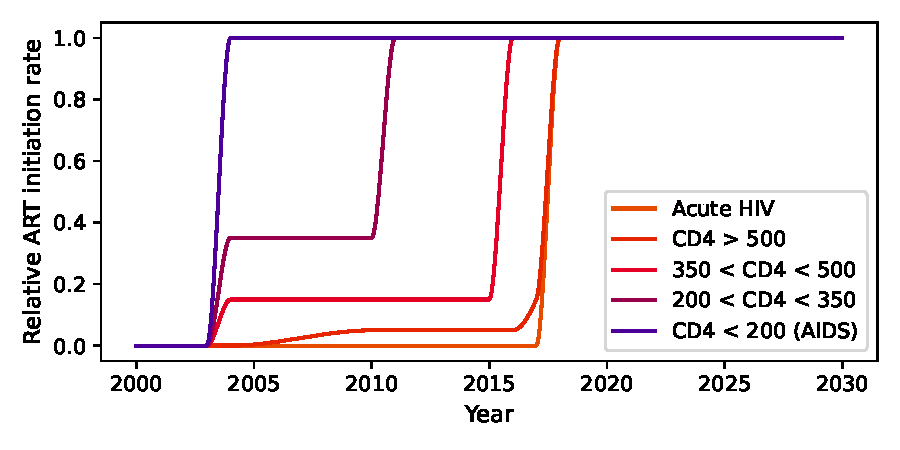
\includegraphics[scale=\fitscale]{art.elig}
  \caption{Modelled relative rates of ART initiation by HIV stage,
    reflecting eligibility changes over time}
  \label{fig:art.elig}
\end{figure}
%---------------------------------------------------------------------------------------------------
\paragraph{Availability and Initiation}
ART first became available in Eswatini in late 2003
via a one-hospital pilot project \cite{NERCHA2012rep}.
Early ART scale-up was modest, with 31 facilities offering ART by the end of 2009 \cite{CDC2013art};
however, this number increased rapidly
to 110 facilities by the end of 2011 \cite{NERCHA2012rep}.
Phase~1 of MaxART (2011--2014) sought to
further increase ART coverage among eligible PLHIV \cite{MaxART1},
including decentralization to lower level facilities,
bringing the total number of facilities to 170 by 2015 \cite{EswMOH2015rep}.
Finally, national adoption of \shortquote{Test and Start} in 2017
likely further reduced delays in ART initiation,
while loss to follow-up was reduced throughout the years of ART scale-up \cite{MaxART2}.
\par
Considering these data, we modelled the yearly ART initiation rate among eligible diagnosed PLHIV as:
effectively $\tau = 0$ in 2003, gradually increasing to 1.5~(0.5,~3.0) by 2010;
then to 9~(6,~12) by 2012; and stabilizing at 12 by 2018.
This maximum rate of $\tau = 12$ corresponds to
a mean effective delay of one month between diagnosis and ART initiation;
this value was chosen in part to avoid numerical instability
when solving the model with very high rates.
%---------------------------------------------------------------------------------------------------
\paragraph{Group Differences}
In 2011, conditional ART coverage (among diagnosed) was greater among men \vs women
(Table~\ref{tab:targ.cascade}),
suggesting greater ART initiation among men \vs women.
Yet, unconditional ART coverage (among PLHIV, regardless of diagnosis)
were approximately equal (31.4 and 33.2\%, respectively),
and so conditional differences may be explained by the fact that
women were more likely to be diagnosed at an earlier HIV stage via antenatal care,
and thereafter not yet eligible for ART.
Thus, we assumed no differences in ART initiation among men \vs women.
A similar mechanism could partially explain
differences in conditional coverage between FSW \vs women overall (36.9 \vs 48.0\%),
as FSW were more slightly likely to know their status (74.1 \vs 69.1\%).
However, FSW face unique barriers to accessing ART
related to stigma and material insecurity \cite{Lancaster2016sr};
as such, we sampled a relative rate for ART initiation among FSW from [0.5,~1] (uniform prior).
% TODO: (?) remove in later years?
%---------------------------------------------------------------------------------------------------
\subsubsection{ART Failure}\label{mod.par.cascade.fail}
% TODO: (~) add Jobanputra2015
The modelled virally un-suppressed state ($c=5$) reflects any combination of
treatment failure (\ie due to resistance mutations),
discontinuation, or loss to follow-up (LTFU) after achieving viral suppression.
The model does not explicitly simulate emergence and/or transmission of drug resistance,
nor multiple unique ART regimens.
As of 2016, resistance mutations to at least 1 of 3 drugs in combination regimens
were identified in 10\% ART-naive PLHIV in Eswatini,
and 16\% PLHIV with prior ART exposure \cite{WHO2021dr}.
However, the extent to which these individual mutations can cause
complete treatment failure remains unclear. % TODO: (~) SM or RK can help?
Additionally, while transmissible resistance mutations could become more prevalent over time,
emergence of new drugs can combat the population-level impacts of this resistance \cite{Hauser2019}.
\par
All available data suggests that retention in ART care
--- \ie not discontinued or LTFU ---
has improved over time in Eswatini \cite{NERCHA2014garp,NERCHA2018rep,SHIMS2}.
Assuming an exponentially-distributed retention time
(consistent with inherent compartmental modelling assumptions),
we averaged the available data \cite[Table~6]{NERCHA2018rep}
to calculated the effective yearly ART attrition rate as:
16.5\% in 2008, 13.8\% in 2010, 14.1\% in 2012, and 8.3\% in 2014.
One-year LTFU was reported as 1\% in 2016 \cite{SHIMS2},
but it's not clear whether this definition was consistent with the earlier estimates.
Many measures of LTFU may also overestimate true LTFU
by failing to account for transfers between clinics and deaths \cite{Fox2018,Wilkinson2015};
it's not clear whether the reported measures for Eswatini account for transfers or deaths.
\par
LTFU was estimated to be 1.3 times higher among men \vs women in South Africa \cite{Fox2018},
which would be consistent with observed lower viral suppression among men \vs women on ART
in Eswatini (Table~\ref{tab:targ.cascade}) \cite{Fox2018}.
The same study estimated that LTFU did not significantly differ
by the modelled CD4-strata \cite{Fox2018}.
No estimates of LTFU were available for FSW specifically in Eswatini,
but among 354 FSW on ART in \cite{EswIBBS2022} (2021),
103 knew the results of viral load monitoring in p12m,
of whom only 8 self-reported undetectable viral load.
Such data may again reflect the unique barriers to accessing ART faced by FSW \cite{Lancaster2016sr}.
\par
Considering all of the above data,  assumed:
a yearly rate of viral un-suppression $\zeta$ among non-FSW women of
15\% until 2010, decreasing to 5\% by 2018;
plus relative rates for men and FSW: [1,~1.5] (uniform priors).
%---------------------------------------------------------------------------------------------------
\subsubsection{Viral Re-suppression}\label{mod.par.cascade.retx}
The rate of viral re-suppression $\sigma'$ aims to reflect the average delay associated with
the steps of switching regimens (in case of treatment failure), or
the steps of re-engaging in HIV care (in case of LTFU).
\par
For treatment failure, viral un-suppression must first be identified.
Availability of viral load monitoring in Eswatini was limited until at least 2010 \cite{EswMOH2010gui},
but incorporated into standard of care by 2015 (yearly testing) \cite{EswMOH2015gui}.
Without viral load testing, treatment failure can still be indicated clinically \cite{EswMOH2010gui}.
After suspecting treatment failure,
at least three months of additional monitoring is typically required
to rule-out issues of adherence \cite{EswMOH2010gui,EswMOH2015gui,EswMOH2018gui},
before another regimen is started.
Moreover, second/third-line regimen options
were limited in Eswatini until at least 2014 \cite{Jobanputra2015,NERCHA2014nsf}.
Upon switching to an improved regimen,  assume that viral suppression occurs
at the same rate as among ART-naive PLHIV (see \sref{mod.par.art}).
\par
For LTFU, no data directly indicate the average duration out of care in Eswatini.
A recent model-based analysis of Kenyan data \cite{Bakoyannis2020} suggests
an average between 8 months and 2 years.
Considering large-scale, multisectorial efforts to improve ART care in Eswatini,
it is likely that duration out of care has declined since 2010.
Thus,  sampled the initial rate of viral re-suppression $\sigma'$ from
a gamma prior with 95\% [0.5,~1.0], which increased by a factor of 1.5 over 2010--2018.
We assumed no differences between groups.

%===================================================================================================
\subsection{Risk Differences Within Sex Work}\label{mod.par.fsw}
Compartmental HIV transmission models which include FSW
have rarely sub-stratified FSW (besides age) \cite{Knight2022sr,Cremin2017,Low2015,Shannon2015},
such as to reflect differential HIV risk or distinct typologies of sex work
\cite{Blanchard2008,Scorgie2012};
yet such heterogeneities may influence transmission dynamics.
Our model structure (Figure~\ref{fig:model.risk})
was designed to capture \emph{within}-FSW risk heterogeneity.
The objective of the following analysis was therefore to parameterize higher \vs lower risk sex work.
For this analysis, we used individual-level data from
two biobehavioural surveys among Swati FSW in
2011 \cite{Baral2014,Yam2013cond} (N = 325) and 2014 \cite{EswKP2014} (N = 781).
More details about each study are given in \sref{mod.par.data}.
\par
Based on community input,%
\footnote{Personal communication: Lungile Khumalo, \emph{Voice of Our Voices}, Eswatini}
we conceptualized risk differences within sex work as transient periods of higher \vs lower risk,
rather than distinct types of sex worker.
As such, we modelled rapid turnover between higher and lower risk FSW (see \sref{mod.par.turn}),
and distinguished these states via the total numbers of clients in p1m.
Specifically, we stratified survey respondents into the top 20\% / bottom 80\%
in total numbers of new and regular clients reported for p1m.
We then summarized key variables within the two strata (Table~\ref{tab:fsw.ratios})
and estimated the ratio of means per \cite{Hauschke1999}.
We repeated this analysis using 2011, 2014, and combined datasets.
\par
Years selling sex, non-paying partners, condom use, anal sex, and HIV status (2011 data only)
did not differ substantially between strata,
while reported numbers of clients and STI symptoms did.
We sampled reported numbers of clients in p1m from gamma distributions with $\alpha = 25$,
reflecting an assumption of mean / 5 = standard deviation;
means were specified as:
14 and 21 for new and regular clients in higher risk sex work, and
3.5 and 6 for new and regular clients in lower risk sex work.
We further use data in Table~\ref{tab:fsw.ratios} regarding:
partners and clients in \sref{mod.par.pnum},
STI symptoms in \sref{mod.par.beta.gud},
condom use in \sref{mod.par.tm.condom},
anal sex in \sref{mod.par.fsex},
years selling sex in \sref{mod.par.turn}.
% TODO: (?) anal sex declining?
\begin{table}
  \centering
  \caption{Ratios of variables among higher \vs lower risk FSW in Eswatini}
  \label{tab:fsw.ratios}
  \begin{tabular}{llRcRcRc}
  \toprule
  & & \multicolumn{2}{c}{Higher} & \multicolumn{2}{c}{Lower} & \multicolumn{2}{c}{Ratio} \\
  \cmidrule(rl){3-4}\cmidrule(rl){5-6}\cmidrule(rl){7-8}
  Year & Variable & mean & (range) & mean & (range) & mean & (95\%~CI) \\
  \midrule 2011
  & Age                                  & 24.5 &  (17, 41)  & 26.6 & (16, 49) & 0.92 & (0.87, 0.98) \\
  & Years selling sex                    & 4.82 &  (0, 18)   & 5.76 & (0, 30)  & 0.84 & (0.63, 1.06) \\
  & Non-paying partners p1m              & 1.32 &   (0, 5)   & 1.45 &  (0, 6)  & 0.91 & (0.71, 1.12) \\
  & New clients p1m                      & 18.9 &  (0, 60+)  & 3.87 & (0, 15)  & 4.87 & (3.55, 6.27) \\
  & Regular clients p1m                  & 23.9 &  (3, 60+)  & 5.71 & (0, 20)  & 4.19 & (3.40, 5.04) \\
  & Non-paying partner condom use\tn{a}  & 0.51 &    ---     & 0.49 &   ---    & 1.04 & (0.74, 1.39) \\
  & New client condom use\tn{a}          & 0.93 &    ---     & 0.87 &   ---    & 1.07 & (0.98, 1.17) \\
  & Regular client condom use\tn{a}      & 0.78 &    ---     & 0.83 &   ---    & 0.94 & (0.80, 1.08) \\
  & Any anal sex p1m\tn{a}               & 0.37 &    ---     & 0.47 &   ---    & 0.79 & (0.50, 1.11) \\
  & Any STI symptoms p12m\tn{a}          & 0.60 &    ---     & 0.48 &   ---    & 1.24 & (0.95, 1.57) \\
  & HIV status\tn{ab}                    & 0.72 &    ---     & 0.70 &   ---    & 1.03 & (0.85, 1.22) \\
  \midrule 2014
  & Age                                  & 27.1 &  (18, 44)  & 27.6 & (18, 50) & 0.98 & (0.95, 1.01) \\
  & Years selling sex                    & 6.12 &  (0, 22)   & 6.44 & (1, 26)  & 0.95 & (0.83, 1.08) \\
  & Non-paying partners p1m              & 1.43 &  (0, 17)   & 1.15 & (0, 10)  & 1.25 & (0.91, 1.61) \\
  & New clients p1m                      & 12.2 &  (0, 60+)  & 3.35 & (0, 16)  & 3.65 & (3.10, 4.23) \\
  & Regular clients p1m                  & 20.0 &  (0, 60+)  & 6.21 & (0, 20)  & 3.22 & (2.89, 3.58) \\
  & Non-paying partner condom use\tn{a}  & 0.71 &    ---     & 0.83 &   ---    & 0.85 & (0.73, 0.98) \\
  & New client condom use\tn{a}          & 0.89 &    ---     & 0.89 &   ---    & 1.00 & (0.93, 1.07) \\
  & Regular client condom use\tn{a}      & 0.82 &    ---     & 0.87 &   ---    & 0.94 & (0.86, 1.02) \\
  & Any anal sex p1m\tn{a}               & 0.13 &    ---     & 0.08 &   ---    & 1.69 & (0.93, 2.70) \\
  & Any STI symptoms p12m\tn{a}          & 0.30 &    ---     & 0.22 &   ---    & 1.34 & (0.98, 1.77) \\
  \midrule Both
  & Age                                  & 26.2 &  (17, 44)  & 27.3 & (16, 50) & 0.96 & (0.93, 0.99) \\
  & Years selling sex                    & 5.63 &  (0, 20)   & 6.27 & (0, 30)  & 0.90 & (0.80, 1.01) \\
  & Non-paying partners p1m              & 1.39 &  (0, 17)   & 1.25 & (0, 10)  & 1.12 & (0.90, 1.35) \\
  & New clients p1m                      & 14.2 &  (0, 60+)  & 3.53 & (0, 20)  & 4.03 & (3.45, 4.63) \\
  & Regular clients p1m                  & 21.2 &  (0, 60+)  & 6.05 & (0, 20)  & 3.51 & (3.18, 3.85) \\
  & Non-paying partner condom use\tn{a}  & 0.62 &    ---     & 0.71 &   ---    & 0.88 & (0.76, 1.01) \\
  & New client condom use\tn{a}          & 0.90 &    ---     & 0.88 &   ---    & 1.02 & (0.96, 1.08) \\
  & Regular client condom use\tn{a}      & 0.80 &    ---     & 0.86 &   ---    & 0.94 & (0.87, 1.01) \\
  & Any anal sex p1m\tn{a}               & 0.19 &    ---     & 0.19 &   ---    & 1.01 & (0.70, 1.36) \\
  & Any STI symptoms p12m\tn{a}          & 0.40 &    ---     & 0.30 &   ---    & 1.33 & (1.08, 1.61) \\
  & HIV status\tn{ab}                    & 0.75 &    ---     & 0.69 &   ---    & 1.07 & (0.90, 1.27) \\
  \bottomrule
\end{tabular}
\floatfoot{
  Higher / Lower: top 20\% / bottom 80\% by total clients p1m;
  \tnt[a]{proportion of respondents};
  \tnt[b]{2011 data only (serologic HIV status)}.}

\end{table}

%===================================================================================================
\subsection{Wider Population: Bias Adjustment}\label{mod.par.wp}
We stratified the remaining women and men (besides FSW and clients)
by numbers of partners in the past 12 months (p12m): 0--1 and 2+.
The 2006-07 DHS \cite{SDHS2006}, 2011 SHIMS \cite{SHIMS1}, and 2016-17 SHIMS2 \cite{SHIMS2} surveys
provide the numbers of respondents who reported 2+ partners in the past 12 months (p12m):
13.5, 18.2, 14.5\% among men, and 1.6, 3.8, 4.1\% among women, respectively.%
\footnote{From
  Tables~14.7.1 and 14.7.2 (ages 15-49) in \cite{SDHS2006},
  Table~3 (ages 18-49) in \cite{SHIMS1},
  Table~15.3.A (ages 15+) in \cite{SHIMS2},
  with manual adjustment for survey skip patterns in \cite{SDHS2006,SHIMS2}.}
However, such reports are likely substantially biased by
social desirability bias due to the face-to-face interview format
\cite{Konings1995,Plummer2004,Gregson2004,Behanzin2013}.
Moreover, these data do not provide information on the \emph{types} of partners reported
--- \ie those reporting 1 partner in p12m
are not necessarily in a main/spousal (vs casual) partnership,
and neither are those reporting 2+ partners in p12m.
Here we develop and apply a new method to adjust for these potential reporting biases,
and simultaneously estimate the numbers of main/spousal and casual partners among each stratum.
The results of these analyses then directly inform
activity group sizes in \sref{mod.par.size.wp} and
numbers of partners in \sref{mod.par.pnum.msc}.
%---------------------------------------------------------------------------------------------------
\subsubsection{Reported Partner Numbers}\label{mod.par.wp.data}
Both the 2006 DHS \cite[Tables 14.6.1 and 14.6.2]{SDHS2006}
and 2016-17 SHIMS \cite[Tables 15.4.A and 15.4.B]{SHIMS2}
summarize the numbers of women and men by partners in p12m \emph{and} by marital/union status,
but summaries are stratified by each factor separately, not jointly.
However, making the following assumptions,
we estimated the jointly-stratified proportions of individuals.
Let $W_{2+}$, $W_{1}$, and $W_{0}$ denote women reporting 2+, 1, and 0 partners, respectively,
and likewise with $M_{2+}$, $M_{1}$, $M_{0}$ for men (all partners reflect p12m).
The assumptions were:
\begin{itemize}
  \item $W_{2+}$ included all women in non-polygynous unions (married or cohabiting)
  reporting sex with a ``casual'' (non-marital, non-cohabiting) partner
  \item $M_{2+}$ included all men in polygynous unions,
  plus all men in non-polygynous unions reporting sex with a casual partner
  \item the remaining $W_{2+}$ and $M_{2+}$ formed only casual partnerships
  \item all women and men in non-polygynous unions
  reporting no sex with a casual partner reported 1 partner ($W_{1}$ and $M_{1}$)
  \item the remaining $W_{1}$ and $M_{1}$ formed only casual partnerships
\end{itemize}
Figure~\ref{fig:xwp} illustrates the resulting
proportions of women and men in each union / partners in p12m stratum
in 2006-07 \sfref{fig:xwp.2006} and 2016-17 \sfref{fig:xwp.2016}.
\begin{figure}
  \centering
  \begin{subfigure}{0.7\linewidth}
    \centering
    \includegraphics[width=\linewidth]{xwp.2006}
    \caption{2006-07 \cite{SDHS2006}}
    \label{fig:xwp.2006}
  \end{subfigure}
  \begin{subfigure}{0.7\linewidth}
    \centering
    \includegraphics[width=\linewidth]{xwp.2016}
    \caption{2016 \cite{SHIMS2}}
    \label{fig:xwp.2016}
  \end{subfigure}
  \begin{subfigure}{0.7\linewidth}
    \centering
    \includegraphics[width=\linewidth]{xwp.adj}
    \caption{Adjusted (mean)}
    \label{fig:xwp.adj}
  \end{subfigure}
  \caption{Reported proportions of women and men aged 15--49,
    stratified by union status and numbers of partners in the past 12 months}
  \label{fig:xwp}
\end{figure}
%---------------------------------------------------------------------------------------------------
\subsubsection{Bias Adjustment: Rationale}\label{mod.par.wp.rat}
We were motivated to examine potential reporting bias because
$M_{2+}$ is consistently much greater than $W_{2+}$.
In fact, this difference is common in surveys \cite{Todd2009,Higgins2010},
and could be explained by either:
(a) a small number of women with many partners,
such as FSW, who may also not be reached by the survey,
or who may not fully report partner numbers;
(b) over-reporting of partnerships by men; or
(c) under-reporting of partnerships by women.
Further stratification of women reporting 2+ partners in \cite[Table~14.7.1]{SDHS2006}
revealed that 94\% reported exactly 2 whereas 6\% reported 3+,
suggesting that explanation (a) is less likely unless
women with 3+ partners are under-reported or indeed missing from the survey.
\par
\citet{Gregson2002bias} (Zimbabwe), \citet{Nnko2004} (Tanzania) and \citet{Clark2011} (Kenya)
explored explanations (b) and (c) through measures of consistency; their results suggested that
under-reporting of non-spousal partnerships by women (c) was more likely,
perhaps due to social norms and pressures.
Such norms in Eswatini are explored in \cite{Ruark2014,Fielding-Miller2016,Ruark2019,Pulerwitz2021}.
In fact, a review comparing computer-based tools \vs face-to-face interviews
for surveying sexual behaviour \cite{Langhaug2010} found that
\emph{both} women and men may under-report sexual partners, but women more so.
A notable 2008 study in Benin \cite{Behanzin2013} found that
7 times as many married women (21 \vs 3\%) and 3 times as many married men (53 \vs 18\%)
reported any extramarital sex in p12m
in a survey via anonymous polling booth \vs face-to-face interview.
Similarly, 5 times as many unmarried women (13.5 \vs 2.8\%) reported
exchanging sex for money, gifts or favours in p12m, while
4 times as many unmarried men (62 \vs 14\%) reported non-transactional sex with a women in p12m.
Such findings were similar to those from Zimbabwe (1990s) \cite{Gregson2002bias}.
%---------------------------------------------------------------------------------------------------
\subsubsection{Bias Adjustment: Approach}\label{mod.par.wp.appr}
To account for the above potential reporting biases
and qualitative insights from \cite{Ruark2014,Fielding-Miller2016,Ruark2019,Pulerwitz2021},
We modelled the adjusted proportions of Swati women and men
in each union / partners in p12m stratum as follows.
Let $W_{s1}$ and $W_{u1}$ denote sub-proportions of $W_{1}$ who are single and in a union, respectively,
and likewise for $W_{s2+}$, $W_{u2+}$, $M_{s1}$, $M_{u1}$, $M_{s2+}$, and $M_{u2+}$.
Further, let $W_{s1}$ denote the reported proportion of women (average of 2006-07 and 2016-17),
\vs $W'_{s1}$ denoting the adjusted proportion.
We assumed that a faction of $W_{0}$ belongs in $W'_{s1}$
--- \ie a fraction of women reporting 0 partners in p12m truly had 1 casual (non-main/spousal) partner.
We modelled this relationship through an odds ratio $\varphi_{W,s1:0}$,
which is roughly equivalent in interpretation to
the proportion ratios estimated by \citet{Behanzin2013}:%
\footnote{Odds ratios ensure no proportions become greater than one or negative.}
\begin{equation}\label{eq:wp.or}
  \varphi_{Ws1:0} = \frac{W'_{s1}}{W'_{0}} \bigg/ \frac{W_{s1}}{W_{0}}
\end{equation}
We defined similar odds ratios $\varphi_{Ws2+:s1}$, $\varphi_{Wu2+:u1}$,
$\varphi_{Wu1:0}$, $\varphi_{Wu1:s1}$, and $\varphi_{Wu2+:s2+}$, and likewise for men.
These strata and the corresponding adjustments / reallocations of women
from reported to adjusted strata are illustrated in Figure~\ref{fig:model.nsw.adj}.
To resolve the adjusted values $W'$ then requires
solving the (nonlinear) system of 6 equations corresponding to the 6 odds ratios $\varphi$,
subject to $\sum_i W'_i = 1$ and $0 \le W'_i < 1$.
An exact solution is not guaranteed,
but the sum squared error from all equations can be minimized.
The odds ratios $\varphi$ were then defined as follows, including sampling distributions.
\begin{figure}
  \centering
  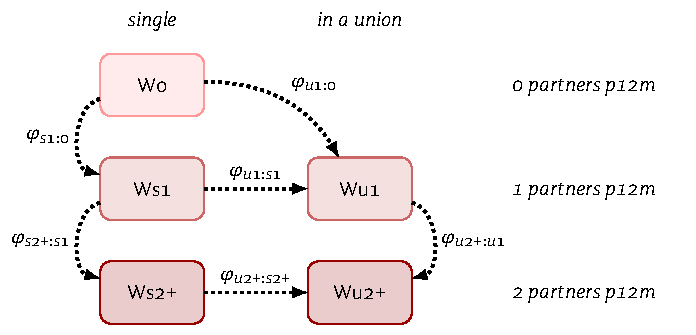
\includegraphics[scale=.8]{diag.nsw.adj}
  \caption{Illustration of how the proportions of women (and equivalently men)
    are adjusted / reallocated between union / partners in p12m strata
    based on odds ratios $\varphi$}
  \label{fig:model.nsw.adj}
  \floatfoot{
    p12m: within the past 12 months;
    W0: 0 partners in p12m;
    Ws1: single (not married/cohabiting) and 1 partner in p12m;
    Wu1: in a union (married/cohabiting) and 1 partner in p12m;
    Ws2+: single and 2+ partners in p12m;
    Wu2+: in a union and 2+ partners in p12m.
    $\varphi$: odds of truly being in the second (arrowhead) \vs first (tail) group.}
\end{figure}
%---------------------------------------------------------------------------------------------------
\paragraph{Union Status}
We assumed that under-reporting of main/spousal partnerships was minimal,
but that some ``main'' partnerships may not be captured in
the definition ``married/cohabiting'' from \cite{SDHS2006,SHIMS2};
thus $\varphi_{u1:0}$, $\varphi_{u1:s1}$, and $\varphi_{u2+:s2+}$
would be small but greater than 1
(horizontal transitions in Figure~\ref{fig:model.nsw.adj}).
Moreover, based on the median age of marriage, 23--29 \cite{SDHS2006},
approximately half of respondents aged 15--49 would have been married,
whereas only 28--39\% of women and men reported being in a union
(Figure~\ref{fig:xwp.2006}~and~\ref{fig:xwp.2016}),
although some marriages end in divorce/widowing \cite{SDHS2006}.
Thus, we sampled each of $\varphi_{u1:0}$, $\varphi_{u1:s1}$, and $\varphi_{u2+:s2+}$
from $1+\opname{Gamma}(\alpha,\beta=1)$
with $\alpha=.5$ for women and $\alpha=.3$ for men,
yielding mean (95\%~CI): 1.50~(1.00,~3.51) and 1.30~(1.00,~2.90), respectively.
%---------------------------------------------------------------------------------------------------
\paragraph{Partner Numbers}
Next, regarding partner numbers,
we defined $\varphi_{s1:0}$, $\varphi_{s2+:s1}$, and $\varphi_{u2+:u1}$ as follows
(vertial transitions in Figure~\ref{fig:model.nsw.adj}).
The median age of first sex in Eswatini was
approximately 18 for women and 19.5 for men \cite{SDHS2006}.
Thus, the 31--36\% of women and 34--41\% of men aged 15--49 reporting no partners in p12m
(Figure~\ref{fig:xwp.2006}~and~\ref{fig:xwp.2016}) is likely overestimated,
although some individuals may be abstinent in p12m following sexual debut.
We assumed that women had 3 and men had 2 times the odds of
actually having 1 casual partner in p12m while reporting no partners.
Thus, we sampled $\varphi_{s1:0}$ from $1+\opname{Gamma}(\alpha,\beta=1)$
with $\alpha=2$ for women and $\alpha=1$ for men,
yielding mean (95\%~CI): 3.00~(1.24,~6.57) and 2.00~(1.03,~4.69), respectively.
Drawing on \cite{Behanzin2013}, we assumed that ``single'' women and men (not married/cohabiting)
were less likely to report multiple partners in p12m, but women more so.
Thus, we sampled $\varphi_{s2+:s1}$ from $1+\opname{Gamma}(\alpha,\beta=1)$
with $\alpha=4$ for women and $\alpha=1$ for men,
yielding 5.00~(2.09,~9.77) and 2.00~(1.03,~4.69).
We made a similar assumption about married/cohabiting women and men,
with the same odds for men, but even greater odds of non-reporting among women.
We sampled $\varphi_{u2+:u1}$ from $1+\opname{Gamma}(\alpha,\beta=1)$
with $\alpha=6$ for women and $\alpha=1$ for men,
yielding 7.00~(3.20,~12.67) and 2.00~(1.03,~4.69).
%---------------------------------------------------------------------------------------------------
\subsubsection{Bias Adjustment: Results}\label{mod.par.wp.res}
The mean resulting adjusted proportions $W'$ and $M'$
from solving the system with the assumed odds ratios $\varphi$
are illustrated in Figure~\ref{fig:xwp.adj}, which can be compared to
the reported proportions in \sfref{fig:xwp.2006}~and~\sfref{fig:xwp.2016}.
Figure~\ref{fig:xwp.adj.dens} also illustrates the empiric density distributions
for each element $W'_{i}$ and $M'_{i}$.
Numerically, the mean (95\%~CI) estimates were:
\begin{itemize}
  \item $W'_{0} = 17~(9,~27)$\% of women and $M'_{0} = 25~(13,~35)\%$ of men had 0 partners in p12m
  \item $W'_{1} = 66~(57,~75)$\% of women and $M'_{1} = 49~(37,~61)\%$ of men had 1 partners in p12m
  \item $W'_{2+} = 17~(10,~27)$\% of women and $M'_{2+} = 26~(15,~44)$\% of men had 2+ partners in p12m
  \item $W'_{u1} / W'_{01} = 38~(21,57)$\% women and $M'_{u1} / M'_{01} = 35~(23,~50)$\% men
    with 0--1 partners in p12m were in a main/spousal partnership
  \item $W'_{s1} / W'_{01} = 41~(19,65)$\% women and $M'_{s1} / M'_{01} = 31~(15,~55)$\% men
    with 0--1 partners in p12m were in a single casual partnership
  \item $W'_{u2+} / W'_{2+} = 32~(9,55)$\% women and $M'_{u2+} / M'_{2+} = 38~(13,~62)$\% men
    with 2+ partners in p12m were in a main/spousal partnership,
    and the rest had only casual partnerships.
\end{itemize}
\begin{figure}
  \centering
  \includegraphics[width=.8\linewidth]{xwp.adj.distr}
  \caption{Density distributions for adjusted proportions of women and men aged 15--49,
    stratified by union status and numbers of partners in the past 12 months}
  \label{fig:xwp.adj.dens}
\end{figure}

%===================================================================================================
\subsection{Activity Group Sizes}\label{mod.par.size}
We model population sizes of all activity groups as proportions of the total population,
which are assumed to remain roughly constant.
Individuals can, however, move between groups (see \sref{mod.par.turn.act})
--- \ie groups are open populations ---
and disproportionate mortality due to HIV between groups
may cause higher risk groups to shrink over time.
Overall population growth is discussed in \sref{mod.par.turn.bd}.
%---------------------------------------------------------------------------------------------------
\subsubsection{Female Sex Workers}\label{mod.par.size.fsw}
The proportion of women who report sex work in national demographic and health surveys
is generally considered unreliable due to social desirability bias,
particularly if the survey is face-to-face and household-based
\cite{Konings1995,Gregson2002bias,Gregson2004,Lowndes2012,Behanzin2013}.
Therefore, FSW population size estimates require
targeted surveys and unique methodologies \cite{UNAIDS2010kps,Abdul-Quader2014}.
In both \cite{EswKP2014} and \cite{EswIBBS2022}, the Swati FSW population size
was estimated using a combination of
unique object method, service multiplier method, prior survey participation,
and network scale-up method (NSUM) \cite{UNAIDS2010kps}.
In 2011 \cite{EswKP2014}, regional FSW population size estimates
ranged from 0.7\% to 6.5\% of all women,
with overall population-weighted mean across regions of 2.9\%;
in 2021 \cite{EswIBBS2022}, the mean (95\%~CI) estimates were 2.43~(1.17,~5.02)\%.
To reflect this uncertainty in the model, we fit a BAB distribution
such that 95\% of the probability fell between 0.7\% and 6.5\%,
and used as the prior distribution for the proportion of women who are FSW.
Then, following the analysis in \sref{mod.par.fsw},
we fixed the proportion of all FSW in the higher risk FSW group at 20\%,
and likewise the lower risk group at 80\%.
%---------------------------------------------------------------------------------------------------
\subsubsection{Clients of FSW}\label{mod.par.size.cli}
Similar to FSW, household-based surveys are not considered reliable data sources
for estimating the population size of clients of FSW \cite{Behanzin2013}.
However, few surveys are designed to reach clients of FSW,
and no direct estimates of FSW size exist for Eswatini.
So, we use a common approach for inferring the FSW client size \cite{Cote2004},
similar to the ``multiplier method'' \cite{Morison2001}.
Given the FSW population proportion $P_{\txc{fsw}}$,
the average number of yearly new and regular sex work clients per FSW $\bar{Q}_{\,\txc{fsw}}$,
the frequency of sex per partnership-year $F_{\txc{sw}}$, and
the average total number of yearly sex acts per client
$\bar{Q}_{\,\txc{Cli}} F_{\txc{sw}}$,
we define the total client population $P_{\txc{cli}}$ as:
\begin{equation}
  P_{\txc{cli}} = \frac{P_{\txc{fsw}}\,\bar{Q}_{\,\txc{fsw}}\,F_{\txc{sw}}}
                                            {\bar{Q}_{\,\txc{cli}}\,F_{\txc{sw}}}
\end{equation}
Then, as with FSW, the proportion of total clients in the higher risk client group
is defined as 20\% of all clients, and likewise for the lower risk group at 80\%.
Using $\bar{Q}_{\,\txc{fsw}}$, $\bar{Q}_{\,\txc{cli}}$, and $F_{\txc{sw}}$
as defined below in \sref{mod.par.pnum.sw}, the prior client population size $P_{\txc{cli}}$
estimated by this method was 11.6~(2.1,~34.4)\% of men.
%---------------------------------------------------------------------------------------------------
\subsubsection{Wider Population}\label{mod.par.size.wp}
Based on the results of \sref{mod.par.wp},
we defined the sizes of the modelled lower and medium activity groups,
and the average numbers of main/spousal partnerships per person.
We assumed that $W'_{2+}$ and $M'_{2+}$ included FSW and client population sizes, respectively.
Thus, we defined the populations size of medium activity women as
$W_{\txc{m}} = W'_{2+} - W_{\txc{fsw}}$.
Sampling $W'_{2+}$ from a BAB distribution with 95\%~CI (10,~27)\%,
the resulting 95\%~CI for medium activity women $W_{\txc{m}}$ was (6,~25)\% of women.
We then defined the lowest activity women population size as $W_{\txc{l}} = 1 - W'_{2+}$,
representing (72,~90)\% of women.
Since there is greater uncertainty in the client population size,
the same approach for the medium activity men population size could yield negative values.
Instead, we sampled the proportion of medium activity men $M_{\txc{m}}$ directly from
a BAB distribution with 95\%~CI (10,~17)\%, yielding
95\%~CI for $M_{\txc{m}} + M_{\txc{cli}}$ of (14,~52)\% of men,
which is close to (15,~44)\% from $M_{2+}$.
We then defined the lowest activity men were as
$M_{\txc{l}} = 1 - M_{\txc{m}} + M_{\txc{cli}}$,
representing (48,~86)\% of men.

%===================================================================================================
\subsection{Turnover}\label{mod.par.turn}
%---------------------------------------------------------------------------------------------------
\subsubsection{Births \& Deaths}\label{mod.par.turn.bd}
The modelled population considers ages 15--49,
reflecting commonly reported data and the majority of sexual activity.
In the absence of mortality, individuals would therefore
remain within the modelled ``open cohort'' population for 35 years.
The estimated average yearly mortality rate for these ages was 1.44\% around 2006
\cite[Table~15.2]{SDHS2006}.
However, this estimate includes HIV/AIDS-attributable mortality,
which we model separately (see \sref{mod.par.hiv.mort}),
accounting for approximately 64\% of deaths around that time \cite{WHO2006esw}.
Thus, the overall exit rate from the modelled cohort
due to reaching age 50 (``aging out'') and non-HIV-attributable mortality was:
$\mu = 1/35 + (1-.64) 1.44\% = 3.78\%$.
\par
We estimated the rate of entry into the modelled population $\nu$
to fit population size of ages 15--49 in Eswatini \cite{WorldBank},
and approximate population growth rates \cite{UNWPP2019},
given that we model HIV/AIDS-attributable mortality separately.
Specifically, we assumed a population growth rate $g = \nu - \mu$ in the absence of HIV/AIDS of
4\% in 1980, 3\% in 2000, 1.5\% in 2010, and 1.5\% in 2020 (monotonic cubic interpolation).
We sampled $g$ in 2050 from a uniform prior with 95\% CI (0.7\%,~1.5\%),
reflecting uncertainty in estimated projections \cite{UNWPP2019}.
Finally, we calculated the population entry rate as $\nu = g + \mu$.
These parameter values were informally validated by comparison of model outputs with
Swati population sizes for ages 15--49 from \cite{WorldBank}.
The distribution of activity groups among individuals \emph{entering} the model, denoted $E_{si}$,
is different from the distribution among individuals \emph{currently} in the model $P_{si}$,
but $E_{si}$ is computed automatically as described below in \sref{mod.par.turn.act}.
%---------------------------------------------------------------------------------------------------
\subsubsection{Activity Group Turnover}\label{mod.par.turn.act}
In addition to overall population turnover (entry/exit from the open population),
we model movement of individuals between activity groups within the model.
Activity group turnover reflects the fact that risk is not constant over sexual life course,
and reported duration in higher activity contexts can be short \cite{Scorgie2012}.
Previous modelling has shown that activity group turnover (sometimes called ``episodic risk'')
can strongly influence parameter fitting and intervention impact \cite{Henry2015,Knight2020}.
We model turnover from activity group $si$ to $si'$ as a constant rate $\theta_{sii'}$,
which implies an assumption that (in the absence of HIV) duration in group $si$ is
exponentially distributed with mean $D_{si}$ \cite{Roberts2015}:
\begin{equation}\label{eq:model.par.dur}
  D_{si} = \frac{1}{\mu + \sum_{i'}\theta_{sii'}}
\end{equation}
where $\mu$ is the overall exit rate from \sref{mod.par.turn.bd}.
As shown previously \cite{Knight2020}, the relative sizes of each sex-activity group $P_{si}$
can be maintained at fixed values by satisfying the following ``mass-balance'' equation:
\begin{equation}
  \nu P_{si} = \nu E_{si} + \sum_{i'} \theta_{si'i} P_{si'} - \sum_{i} \theta_{sii'} P_{si}
\end{equation}
Specific turnover rates $\theta_{sii'}$ and entrant activity group sizes $E_{si}$
can then be uniquely resolved by specifying
$N_i\,(N_i-1) = 12$ non-redundant and compatible constraints,
where specifying each $D_{si}$ is one such constraint.
% ---------------------------------------------------------------------------------------------------
\paragraph{Selling Sex}
Estimating durations (\eg in sex work) from cross-sectional data
should consider several potential sources of bias \cite{Fazito2012,Knight2023bias},
including distributional, sampling, censoring, and measurement biases.
We previously explored these biases using the 2011 Eswatini FSW survey data \cite{Baral2014}
and inferred adjusted estimates of sex work duration
via a Bayesian Bayesian hierarchical model \cite{Knight2023bias}.
We estimated a mean duration of 4.06~(2.29,~6.34) years,
with durations distributed approximately exponentially
--- compatible with the implicit assumption of compartmental models \cite{Anderson1991}.
Thus, we sampled overall duration in sex work from a gamma prior with 95\%~CI (2.29,~6.34) years.
As noted in \sref{mod.par.fsw}, we conceptualized higher risk sex work as
a transient period, with short duration.
We sampled this duration from a gamma prior with 95\%~CI (2,~12) months.
We then modelled turnover for higher risk sex work as
exclusively coming from / going to lower risk sex work,
including no direct entry from outside the model: $E_{si} = 0$.
By contrast, women entering lower risk sex work could
enter directly from outside the model ($E_{si} > 0$),
and turnover from / to any other activity group.
%---------------------------------------------------------------------------------------------------
\paragraph{Buying Sex}
Data to inform the average duration spent buying sex among clients is limited.
\citet{Fazito2012} estimated mean durations of 4.6--5.5 years
based on studies in Benin \cite{Lowndes2000} and Kenya \cite{Voeten2002}.
\citet[Table~G]{Hodgins2022} also gives pooled estimates for
the proportions of men in Sub-Saharan Africa
who paid for sex \emph{ever} \vs in \emph{p12m} during 2000--2020.
Estimates ranged from 8.8~(6.5,~11.7)\% of men aged 25--34 who ever bought sex,
to 2.2~(1.5,~3.2)\% of men aged 35--54 who bought sex in p12m.
Based on these data, we defined a gamma prior distribution for
the total duration buying sex with 95\%~CI (4,~15) years.
We conceptualized higher risk clients as a transient period
with the same duration as higher risk sex work,
and assumed an equal pattern of possible turnover between activity groups
among men buying sex as women selling sex.
%---------------------------------------------------------------------------------------------------
\paragraph{Lowest \& Medium Activity Groups}
Data on individual-level changes to numbers of non-sex work partners in p12m
is even more sparse than data related to sex work;
so, it's unclear to what extent individuals move between the lowest and medium activity groups
throughout their sexual life course.
Data from Uganda, Zimbabwe, and South Africa \cite{Todd2009}
suggested that sexual activity (proportion sexually active and mean numbers of partners)
was approximately stable with age (after sexual debut and and before age 49),
with modest trends toward lower activity at older age.
However, these population-level data do not necessarily suggest that
the \emph{same} individuals have multiple partnerships each year.
Reflecting this uncertainty, we sampled
the rate of turnover from medium to lowest activity for both women and men
from a gamma prior with 95\%~CI (5,~50)\% per year.
%---------------------------------------------------------------------------------------------------
\paragraph{Additional Turnover Assumptions}
The above assumptions specify 8 constraints for each sex:
2 durations $D_{si}$, 1 entry rate $E_{si} = 0$, and
5 turnover rates $\theta_{sii'}$ (4 zero, 1 nonzero).
Next, since FSW often enter sex work shortly after sexual debut \cite{Cheuk2020,Ma2020},
and sexual activity is roughly constant or slightly declining with age \cite{Todd2009},
we assumed that $E_{si} = f\,P_{si}$,%
\footnote{Subject to $f \le (\nu - \mu + D_{si}^{-1})\,\nu^{-1}$,
  which can be derived from Eq.~(10) in \cite{Knight2020}.}
with $f = 2$ for lower risk FSW, $f = 1.5$ for lower risk clients,
and $f = 1$ for medium activity women and men (+2~constraints);
then $f < 1$ for the lowest activity women and men is computed automatically.
Finally, since exiting sex work is unlikely to be
an abrupt transition to monogamous or zero sexual activity \cite{Scorgie2012,Learmonth2015},
we further assumed that (50,~90)\% of women exiting sex work
transition to the medium activity group (BAB prior) (+1~constraint);
in the absence of relevant data, we made a similar assumption regarding clients,
with (25,~90)\% former clients transitioning to the medium activity group (+1~constraint).
These $10 < 12$ total constraints then allow two degrees of freedom to resolve
the values of $\theta_{sii'}$ and $E_{si}$.
A non-negative solution to the system of constraints is solved as described in \cite{Knight2020},%
\footnote{Using \hreftt{docs.scipy.org/doc/scipy/reference/generated/scipy.optimize.nnls.html}}
repeated at each timestep since $\nu$ varies with time.

%===================================================================================================
\subsection{Partnership Numbers}\label{mod.par.pnum}
This section summarizes the numbers of partnerships modelled among activity groups.
Similar to group sizes, we draw on the
analysis of FSW data in \sref{mod.par.fsw} and
bias adjustment for wider population in \sref{mod.par.wp},
we well as further adjustments with regards to partnership duration \cite{Knight2023bias}.
%---------------------------------------------------------------------------------------------------
\paragraph{Adjusting for Partnership Duration}
As noted in \sref{mod.foi},
sexual partnerships are usually quantified using a change rate $Q$,
whereas our force of infection equation uses a number of current partners $K$.
Either parameter may be estimated from survey questions like
\shortquote{How many casual sexual partners have you had in the past 12 months?}
However, this estimation must account for both the
recall period $\omega$ (\eg 12 months) and
partnership duration $\delta$ (\eg 6 months) per \cite{Knight2023bias}:
\begin{alignat}{1}
  Q &= \frac{x}{\omega+\delta} \label{eq:x2Q}\\
  K &= \frac{x\delta}{\omega+\delta} = Q\delta \label{eq:x2K}
\end{alignat}
where $x$ is the mean number of partners reported in the recall period.
%---------------------------------------------------------------------------------------------------
\subsubsection{Sex Work Partnerships}\label{mod.par.pnum.sw}
% ---------------------------------------------------------------------------------------------------
\paragraph{Female Sex Workers}
Table~\ref{tab:fsw.ratios} summarizes
the numbers of new and regular clients \emph{per month} reported by Swati FSW,
stratified by higher \vs lower risk per the analysis in \sref{mod.par.fsw}.
These data thus would provide $x$ for $\omega = 1$ month.
However, based on the survey questions,%
\footnote{The survey questions were: \shortquote{In the last 30 days,
  how many (new/regular) clients have you had sex with?}, or similar.}
it's not clear whether these reported partner numbers
represent the numbers of unique men or unique client visits.
\par
We assumed that all \emph{new} clients were one-off visits;
thus the reported partner numbers effectively represented
$1/12$th of the total numbers of yearly partnerships $Q_{\,\txc{swo}}$.
As such, we sampled the yearly rate of occasional sex work partnerships among lower risk FSW
from a gamma distribution with mean (95\%~CI) as 3.5~(2.3,~5.0) $\times$ 12,
and the rate among higher risk FSW from 14~(9,~20) $\times$ 12.
Since each partnership is assumed to include only one sex act,
the partnership duration $\delta_{\txc{swo}}$, frequency of sex $F_{\txc{swo}}$,
and number of concurrent partnerships $K_{\txc{swo}}$ are ill-defined,
but can be defined for convenience as
$\delta_{\txc{swo}} = 1/12$ (years), $F_{\txc{swo}} = 12$ (per year),
and $K_{\txc{swo}} = Q_{\,\txc{swo}} / 12$.
\par
For \emph{regular} sex work partnerships, uncertainties remain regarding
partnership duration $\delta_{\txc{swr}}$ (see \sref{mod.par.pdur}),
frequency of sex per month $F_{\txc{swr}}/12$, and
survey responses $x$ reflecting unique clients or total client visits per month.
If $x$ reflects the numbers of unique clients, then
$Q_{\,\txc{swo}}$ can be defined via \eqref{eq:x2Q} using $x$ directly;
whereas if $x$ reflects the numbers of unique visits, then
$Q_{\,\txc{swo}}$ should be defined using $x/(F_{\txc{swo}}/12)$.
We assumed that $2/3$ \vs $1/3$ of respondents interpreted the question
as in the former \vs latter case, such that:
\begin{equation}\label{eq:x.swr}
  x' = (2/3)\,x + (1/3)\,x/(F_{\txc{swr}}/12)
\end{equation}
Taking $F_{\txc{swr}}/12 = 2$ as the prior mean from \sref{mod.par.fsex},
\eqref{eq:x.swr} simplifies to $x' = \frac{5}{6}\,x$.
Thus, we defined $K_{\txc{swr}}$ via \eqrefs{eq:x2K}{eq:x.swr}, with:
$\omega = 1/12$ (1 month),
$\delta_{\txc{swr}}$ as specified in \sref{mod.par.pdur}, and
$x_{\txc{swr}}$ from the gamma distributions given in \sref{mod.par.fsw}.
% TODO: (*) summarize distributions: K, KF
%---------------------------------------------------------------------------------------------------
\paragraph{Clients}
Across Sub-Saharan Africa, data for clients of FSW on
the number of unique FSW visited and the frequency of sex is sparse.
Among 64 clients in Kenya,
the median number of sex work visits per week was 1.3 (68 per year);
most clients (68\%) had 1--3 regular FSW partners simultaneously, and
visited 0--3 new FSW per year \cite{Voeten2002}.
Among 261 truck drivers at sex work hotspots in Uganda,
the mean number of sexual partners was
7.4 in the past 30 days and 44.7 in the past year \cite{Matovu2012}.
\citet{Johnson2017} modelled yearly sex work visits among South African clients of FSW as
gamma-distributed with age over 10, peaking at 64 visits per year for clients aged 37.
To reflect these data, we specified clients overall to have
mean (95\%~CI) 36~(18,~72) sex acts with FSW per year
($K_{\txc{sw}}\,F_{\txc{sw}}/12$, gamma prior).
Then, the yearly sex acts among lower and higher risk clients are defined such that
higher risk have 2.0~(1.6,~2.5) times the number among lower risk.
Finally, since the distribution of sex acts between new \vs regular sex work partnerships
must match that among FSW, the specific values of $K_{\txc{sw}}$
were computed automatically.
% TODO: (*) summarize distributions: K, KF
%---------------------------------------------------------------------------------------------------
\subsubsection{Main/Spousal \& Casual Partnerships}\label{mod.par.pnum.msc}
Drawing on the results in \sref{mod.par.wp.res},
we defined the numbers of main/spousal and casual partners
among each activity group as follows.
%---------------------------------------------------------------------------------------------------
\paragraph{Main/Spousal Partnerships}
To simplify model fitting, we sampled a common proportion $x$ of
individuals reporting a main/spousal partnership from a BAB distribution with 95\%~CI (25,~50)\%,
applied to all women and men in the lowest activity groups,
as well as all women in the medium activity group.
Then, we used \eqref{eq:x2K} to define $K$ using $\omega = 1$ year and
the main/spousal partnership duration from \sref{mod.par.pdur}.
Since FSW and clients had fewer main/spousal partnerships (see below),
we calculated the proportion of men in the medium activity group having main/spousal partnerships
to balance the total number of main/spousal partnerships among women and men.
%---------------------------------------------------------------------------------------------------
\paragraph{Casual Partnerships}
We similarly defined a common proportion of women and men in the lowest activity groups
reporting casual partnership $x_{\txc{cas}}$ with 95\%~CI (20,~55)\%.
However, the number of casual partnerships among $W_{2+}$ and $M_{2+}$ ramains uncertain.
The analysis in \sref{mod.par.wp} provides no information on these values,
but the number of casual partners in p12m
for the medium activity groups must be at least about 1.5
to ensure these women and men actually have 2+ partners in p12m.
Thus, we sampled the number of casual partners
reported by women in the medium activity group $x$
from a gamma distribution with 95\%~CI (1.2,~2),
and computed $K$ via \eqref{eq:x2K}.
As before, we calculated the numbers of casual partnerships
among men in the medium activity group to balance total casual partnerships.
%---------------------------------------------------------------------------------------------------
\paragraph{Main/Spousal \& Casual Partnerships among FSW \& Clients}
Among Swati FSW, the mean number of total non-paying partners in the past month was
approximately 1--1.5 (Table~\ref{tab:fsw.ratios}),
which may include both main/spousal partners and casual partners.
Among FSW in South Africa \cite{Wells2018} and Kenya \cite{Voeten2007},
while 54 and 72\% (respectively) reported being in a relationship, only 6 and 3\% were married,
although many non-marital partners may still constitute effectively ``main'' partnerships
with respect to condom use and duration.
Thus, we assumed that:
50\% of all FSW reported a main/spousal partner in p12m;
lower risk FSW reported 0.5 casual partners; and
higher risk FSW reported 1.0 casual partners, on average.
\par
Available data suggest that about half of clients also report non-sex work partners,
which are not always distinguished as main/spousal \vs casual partnerships
\cite{Lowndes2000,Santo2005}.
Non-paying partners of FSW are also often clients of other FSW \cite{Voeten2007,Godin2008}.
Yet, clients of FSW also tend to be younger and more likely to be
never/formerly married \vs non-client men \cite{Lowndes2000,Carael2006}.
So, we assumed that clients reported
half the numbers of main/spousal partnerships compared to lowest activity men, and
25--100\% the numbers of casual partnerships compared to medium activity women (uniform prior).
As before, we computed $K$ via \eqref{eq:x2K}
with partnership durations from \sref{mod.par.pdur}.

%===================================================================================================
\subsection{Sex Frequency}\label{mod.par.fsex}
The Eswatini general population data sources \cite{SDHS2006,SHIMS1,SHIMS2}
did not report on frequency of sex. % TODO: (*) SDHS2006: Table 6.10
In South Africa, average numbers of sex acts per week per partnership (non-sex work)
was reported as mean 2.5~(IQR: 1--3) \cite{Delva2013},
with consistent reports across main/spousal partnerships and casual partnerships.
Sex frequency among South Africans per month overall (not per-partnership)
is also summarized in \cite[Figure~3.15]{Shisana2005},
which is roughly consistent with \cite{Delva2013}, but motivates a smaller lower bound.
Median sex frequency per partnership-year in 1998 Rakai, Uganda was
approximately 90 acts with the ``more frequent'' of concurrent partners, and
approximately 20 acts with the ``less frequent'' \cite{Morris2010}.
Considering these data,
we sampled the number of sex acts per year in main/spousal partnerships
from a gamma prior distribution with 95\%~CI (26,~156),
and a relative rate for casual partnerships from $\opname{Unif}(0.5,2)$.
As described in \sref{mod.par.pnum.swx},
we defined $F_{\txc{swo}} = 12$ for occasional sex work partnerships,
and $F_{\txc{swr}} \sim \opname{Unif}(12,36)$ for regular sex work partnerships.
We also constrained samples of $F_{p_{4}}$ such that
higher risk FSW never have commercial sex more than twice daily, on average.
% TODO: (?) Coital frequency is not thought to be influenced by concurrent partnerships \cite{Delva2013}.
%---------------------------------------------------------------------------------------------------
\paragraph{Anal Sex}
Among Eswatini data sources, only \cite{EswKP2014} (FSW, 2014)
counted sex acts separately for anal and vaginal sex.%
\footnote{\citet{Owen2020esw} examined prevalence of anal sex in p1m among Swati FSW in 2011,
  but could not comment on frequency due the survey questions.}
Among all FSW, the proportion of ``average sex acts per week'' that were anal (vs vaginal) was 2.9\%.
However, a previous coital diary study in neighbouring KwaZulu-Natal suggested
much higher proportions were anal \cite{Ramjee1999},
and face-to-face interview survey design may result in under-reporting \cite{Owen2020sr}.
Owen et al. review studies of anal sex in South Africa, and estimate that
0.6--16.5\% of sex acts among the general population are anal \cite{Owen2017}, \vs
2.4--15.9\% among FSW \cite{Owen2020sr}.
To reflect this data, we sampled the proportions of sex acts which are anal
in main/spousal and casual partnerships from
a gamma prior distribution with 95\%~CI (0.6,~16.5)\%,
and a relative proportion in all sex work partnerships from $\opname{Unif}(1,2)$.
%===================================================================================================
\subsection{Partnership Duration}\label{mod.par.pdur}
Eswatini-specific data on partnership duration are lacking.
Moreover, accurate estimation of partnership duration remains challenging even when data exist,
due to censoring, truncation, and sampling biases \cite{Burington2010,Knight2023bias}.
Similar to challenges in estimating sex work duration,
we must distinguish the definition of an ``average partnership'' as
(a) among all partnerships in a population over a given \emph{time period}, \vs
(b) among all partnerships in a population \emph{cross-section}.
Case (b) will be biased by partnership duration,
so the estimated mean duration will longer,
while case (a) reflects an unbiased estimate.%
\footnote{If case (a) durations are exponentially distributed,
  the durations in case (b) will be gamma-distributed with $\alpha = 2, \beta = \lambda$;
  thus the mean duration in case (b) will be $\alpha/\beta = 2\lambda$ (twice as long).}
The difference between the exponential distribution
mean ($1/\lambda$) and median ($\log2/\lambda$) should also be kept in mind.
%---------------------------------------------------------------------------------------------------
\paragraph{Main/Spousal Partnerships}
Detailed data on marriage in Eswatini was only captured in 2006 \cite[Table~6.1]{SDHS2006}.
The median age of first marriage was 24.3 among women and 27.7 among men (26.0 overall).
Approximately 64\% of women and 88\% of men (76\% overall) who were ever married or living together
were in a union at age 50--54.
However, no data indicated whether any respondents had remarried or entered into a secondary union.
Among women aged 40--49, the most recent data on
median age of first marriage and proportions ever remarried were
33 years old and 6.6\% in South Africa,
20.9 and 3.7\% in Lesotho, and 18.7 and 28.4\% in Mozambique \cite{John2022};
such data may not capture non-marital secondary unions.
Thus, we assumed $\rho = {}$5--20\% of unions among EmaSwati aged 50--54 were secondary.
Considering that the modelled population only includes ages 15--49,
we then defined the mean durations of main/spousal partnerships as
$\delta_{\txc{msp}} =  (0.76 - \rho)\,(49 - 26) \in (14.5, 18.5)$ years.
\par
In some models, partnership duration is used to define both
the total numbers of sex acts per partnership and the partnership change rate (see \sref{foi.prop}).
This change rate might be overestimated by the above definition,
since the rate should also consider whether and when
divorced/separated individuals form \emph{new} main/spousal partnerships.
The change rate could even be tied to the modelled baseline and HIV-attributable mortality,
given that the majority of Swati unions ended via spousal death
(83\% of unions among women and 56\% among men by age 50--54) \cite{SDHS2006}.
% TODO: (?) add exit from "k=1" state, rate proportional to HIV-attrib-mort of opposite sex?
For simplicity and consistency with prior approaches,
we used the effective duration of 14.5--18.5 years throughout (uniform prior).
%---------------------------------------------------------------------------------------------------
\paragraph{Casual Partnerships}
No data is available regarding durations of non-marital sexual partnerships in Eswatini,
and regional data on are also limited.
We synthesized the available partnership duration data from
South Africa \cite{Harrison2008,Hargreaves2009,Nguyen2015},
Rural Tanzania \cite{Nnko2004},
and four cities in Kenya, Zambia, Benin, and Cameroon \cite{Ferry2001}.
Based on these data, we defined a gamma prior distribution for
the mean duration of casual partnerships $\delta_{\txc{cas}}$ with 95\%~CI (0.25,~1.5) years,
roughly consistent with prior models \cite{Johnson2009}.
A gamma distribution was chosen \vs uniform or normal
to reflect non-uniform belief while preventing negative values.
%---------------------------------------------------------------------------------------------------
\paragraph{Sex Work Partnerships}
As noted in \sref{mod.par.pnum.swx}, duration of occasional sex work partnerships
is ill defined, but can be defined to comprise a single sex act with
$F_{\txc{swo}}\delta_{\txc{swo}} = 1$.
Data on regular sex work partnerships is severely limited, and
sometimes regular paying clients later become
non-paying emotional partners \cite{Voeten2007,Mbonye2022}.
Based on \cite{Voeten2002}, I defined a gamma prior distribution for
the mean duration of regular sex work partnerships $\delta_{\txc{swr}}$
with 95\%~CI (2,~12) months.

%===================================================================================================
\subsection{Mixing}\label{mod.par.mix}
In addition to more transmission among FSW and their clients
via regular and occasional sex work partnerships
--- which are \emph{only} formed among FSW and clients ---
other types of partnerships may be formed
preferentially between particular activity groups.
For example, FSW and clients may be more likely to form main partnerships
with each other than with other activity groups.
Such preferences are captured in a ``mixing matrix'' $M$, where $M_{pii'}$ denotes
the total number of type-$p$ partnerships formed between groups $i$ and $i'$ in the population
(ignoring sex indices $s,s'$ temporarily)
--- \ie who has sex with whom.
The mixing matrix $M_{pii'}$ must be symmetric,
and have row/column sums equal to the total numbers of partnerships ``offered'' by any group:
$M_{pi} = P_{i} K_{pi}$ (group size $\times$ partnerships per-person).
%---------------------------------------------------------------------------------------------------
\subsubsection{Log-Linear Mixing}\label{mod.par.mix.ll}
Many risk/activity-stratified compartmental transmission models
parameterize mixing via a single parameter $\epsilon \in [0,1]$,
which controls the degree of like-with-like mixing \cite{Nold1980,Garnett1994}.
However, the simplicity of this approach precludes more complex mixing patterns
--- such as preferential mixing among two of four total groups.
A more general approach to mixing is developed in \cite{Morris1991ll}.
This ``log-linear'' approach defines the mixing matrix elements $M_{pii'}$ as follows.
The expected total numbers of partnerships between risk groups under random mixing are defined as:
\begin{equation}\label{eq:mix.rand}
  \Pi_{pii'} = \frac{M_{pi} M_{pi'}}{\sum_{j} M_{pj}}
\end{equation}
Next, a matrix $\Phi_{pii'}$ is defined, representing the odds of
a type-$p$ partnership forming between groups $i$ and $i'$, compared to random mixing.
The matrix $\Phi$ must be symmetric,
and can be estimated directly from the right kind of data
(which is rarely available) \cite{Morris1991ll}.
Then, an initial estimate of $M_{pii'}$ is:
\begin{alignat}{1}
  M_{pii'}^{\,(0)} &= \exp{\left[\log{\left(\Pi_{pii'}\right)} + \Phi_{pii'} \right]} \nonumber\\
                 &= \Pi_{pii'} \exp{\left(\Phi_{pii'}\right)} \label{eq:mix.M0}
\end{alignat}
However, this estimate changes the total numbers of partnerships formed by each group:
$M_{pi}^{\,(0)} \ne \Pi_{pi}$, where
$M_{pi} = \sum_{i'} M_{pii'}$ and $\Pi_{pi} = \sum_{i'} \Pi_{pii'}$.
There is no \textit{a priori} definition of $M_{pii'}$ or adjustment to $\Phi_{pii'}$
that can guarantee the numbers of partnerships will not change.
However, an iterative proportional fitting procedure \cite{Ruschendorf1995}
can resolve an estimate $M_{pii'}^{\,(\infty)}$ that maintains the total numbers of partnerships:
\begin{equation}\label{eq:mix.iter}
  M_{pii'}^{\,(n+1)} = M_{pii'}^{\,(n)} \frac{\Pi_{pf}}{M_{pf}^{\,(n)}}
  \qquad f = \begin{cases}
    ~i  & \txn{if $n$ is even} \\
    ~i' & \txn{if $n$ is odd}
  \end{cases}
\end{equation}
Each step of this procedure can be understood as
a re-scaling of the current estimate $M_{pii'}^{\,(n)}$
row-wise ($i$) or column-wise ($i'$) to match the numbers of partnerships
offered by individuals ($\Pi_{pi}$) or their partners ($\Pi_{pi'}$).
Each row-step re-introduces discrepancies in the columns, and vice versa,
but overall convergence is guaranteed~\cite{Sinkhorn1964}.
\par
In practice, \eqref{eq:mix.iter} adds approximately
one decimal of precision per $2n$ for the $4\times4$ case,
thus 15--20 iterations is often sufficient to come within computational precision limits.
Since the partnerships matrix $M_{pii'}$ should adapt to reflect changes in
group sizes (\eg due to HIV mortality) or
numbers of partnerships offered (\eg see \sref{mod.foi}),
the matrix must be re-computed at every time point.
Thus, the procedure \eqref{eq:mix.iter} could be considered computationally expensive.
However, this approach provides great flexibility and interpretability
to specify complex mixing patterns via the odds matrix $\Phi_{pii'}$.
\par
Two final adjustments are needed for the bipartite (\ie heterosexual) system,
after adding back the sex dimension indices $i \rightarrow si, ~ i' \rightarrow s'i'$.
First, we ensure that $M_{s=s'} = \Pi_{s=s'} = 0$.
Second, for the case when the total numbers of partnerships offered by women and men
do not balance ($\sum_j M_{ps_{1}j} \ne \sum_j M_{ps_{2}j}$),
We revise the denominator of \eqref{eq:mix.rand} to $\sum_{j} \psi_s M_{psj}$,
where $\psi_s$ are weights such that $\sum_s \psi_s = 1$.
Similar to the ``compromise'' parameter $\theta$ in \cite{Garnett1994},
if $\psi = \{1,0\}$, then women's partnership numbers are matched exactly
while men adapt their partner numbers to balance;
and conversely for $\psi = \{0,1\}$.
We fixed $\psi = \{0.5,0.5\}$ for equal adaptation among women and men.
%---------------------------------------------------------------------------------------------------
\subsubsection{Odds of Mixing}\label{mod.par.mix.odds}
Despite the flexibility in the odds of mixing matrix $\Phi_{pii'}$,
and the importance of mixing patterns for transmission dynamics \cite{Garnett1993hiv},
there are limited data to inform mixing patterns for Eswatini.
In Kenya \cite{Voeten2007}, Benin, Guinea, and Senegal \cite{Godin2008}, and Uganda \cite{Mbonye2022},
a disproportionate fraction of non-paying partners of FSW were former and/or current clients.
However, its not clear whether such partnerships reflect main/spousal and/or casual partnerships.
As such, we sampled a common value for both partnership types
$\sim \exp[\opname{Unif}(-2,+2)]$,
applied equally to higher and lower risk FSW and clients.
We further assumed that lowest activity women and men had
greater odds of forming main/spousal partnerships with each other,
based loosely on age cohorting effects \cite{Leclerc-Madlala2008},
observed like-with-like sexual mixing preferences in other contexts
\cite{Morris1991ll,Garnett1993gon,Admiraal2016},
and prior models \cite{Knight2022sr}.
We sampled this odds ratio from an equal prior: $\exp[\opname{Unif}(-2,+2)]$.
We made no further assumptions about preferential mixing (\ie all other elements $\Phi = 0$).
Thus, we assumed that occasional and regular sex work partnerships form
randomly with respect to higher \vs lower FSW and their clients.

